\documentclass[journal, 12pt, onecolumn, draftclsnofoot]{IEEEtran} %JSAC 20'
\usepackage[linesnumbered,vlined,ruled]{algorithm2e}
\usepackage{algorithmic}
\usepackage{etoolbox}
\usepackage{cite}
\usepackage{amsmath,amsthm,amssymb,amsfonts}
\usepackage[dvipsnames]{xcolor}
\usepackage{dcolumn}
\usepackage{graphicx}
\usepackage[utf8]{inputenc}
\usepackage{soul}
\usepackage{mathtools}
\graphicspath{ {./images/} }
\usepackage{tabularx}
%---------------------------------------------------------------%
\newtheorem{definition}{Definition}   % 
\theoremstyle{definition}             % alter theorem style: <definition>
\newtheorem{program}{Program}         % [program]
\newtheorem{assumption}{Assumption}   % [assumption]
\newtheorem{example}{Example}         % [example]
\newtheorem{Algorithm}{Algorithm}     % [algorithm]
\newtheorem{policy}{Policy}           % [policy]
\newtheorem{problem}{Problem}         % [problem]
\theoremstyle{remark}                 % alter theorem style: <remark>
\newtheorem{remark}{Remark}           % [remark]
\theoremstyle{plain}                  % alter theorem style: <plain>
\newtheorem{theorem}{Theorem}         % [theorem]
\newtheorem{lemma}{Lemma}             % [lemma]
\newtheorem{corollary}{Corollary}     % [corollary]
%---------------------------------------------------------------% math symbols
\newcommand{\eq}{=}
\newcommand{\domZ}{\mathbb{Z}_{*}}
\newcommand{\domP}{\mathbb{Z}_{*}}
\newcommand{\vecOne}{\mathbf{1}}
\newcommand{\ind}{\mathbf{I}}
\newcommand{\mat}{\mathbf}
\newcommand{\Poisson}{\text{Poisson}}
\newcommand{\Bernoulli}{\text{Bernoulli}}
\newcommand{\define}{\triangleq}
\newcommand{\leadto}{\Rightarrow}
\newcommand{\vecG}{\boldsymbol}
\renewcommand{\vec}{\mathbf}
\DeclarePairedDelimiter{\set}{\{}{\}}
\DeclarePairedDelimiter{\norm}{|}{|}
\DeclarePairedDelimiter{\Inorm}{\|}{\|_1}
\DeclarePairedDelimiter{\Paren}{\bigg(}{\bigg)}
\DeclarePairedDelimiter{\Bracket}{\bigg[}{\bigg]}
\DeclarePairedDelimiter{\Brace}{\bigg\{}{\bigg\}}
%---------------------------------------------------------------% comments
\newcommand{\fixit}[1]{{\color{red}{#1}}}
\newcommand{\accept}[1]{#1}
\newcommand{\comments}[1]{{\color{blue}{#1}}}
\newcommand{\deny}[1]{\st{#1}}
\newcommand{\delete}[2]{}
\newcommand{\needref}[1]{\text{[#1]}}
%---------------------------------------------------------------% user-defined
\newcommand{\AP}{\dagger}
\newcommand{\ES}{\ddagger}
\newcommand{\apSet}{\mathcal{K}}
\newcommand{\esSet}{\mathcal{M}}
\newcommand{\ccSet}{\mathcal{X}}
\newcommand{\jSpace}{\mathcal{J}}
\newcommand{\Stat}{\mathbf{S}}
\newcommand{\Obsv}{\mathcal{Y}}
\newcommand{\Policy}{\vecG{\Omega}}
\newcommand{\Delay}{\vecG{\mathcal{D}}}
\newcommand{\Baseline}{\vecG{\Pi}}
\newcommand{\algname}{Solver}

\newcommand{\brlatency}{signaling latency}
% \newcommand{\brpoint}{\emph{broadcast point}}
%---------------------------------------------------------------%
\usepackage{fancyhdr}
\pagestyle{fancy}
\fancyhead[LO]{Probationary Report}
% \fancyhead[RO]{Yuncong Hong}

\begin{document}
    \title{
        Distributed Job Dispatching Cooperation in Edge Computing Network with Outdated Information
    }

    \author{
        \begin{tabular}{rl}
            \textbf{Name: }&                Yuncong Hong \\
            \textbf{HKU No.:}&        3030058647 \\
            \textbf{Curriculum:}&           Doctor of Philosophy (4 years) \\
            \textbf{Department:}&           Department of Computer Science \\
            \textbf{Supervisors:}&          Prof. CL Wang and Prof. FCM Lau 
        \end{tabular}
    }

    \maketitle
    \fancypagestyle{firststyle}
    {
        \fancyhf{}
        \fancyhead[LO]{Probationary Report}
    }
    \thispagestyle{firststyle}
    

    \renewcommand{\abstractname}{\vspace{-\baselineskip}}
\begin{abstract}
    \fixit{In this paper,} we consider the distributed job dispatching problem in an edge computing network residing in a Metropolitan Area Network (MAN), where the job arrivals, uploading latency and computation time are all random.
    Specifically, multiple access points (APs) collect jobs from the mobile users, and upload each job to one edge server according to the job type.
    APs and edge servers periodically broadcast their local state information.
    The signaling latency of broadcast information is also random, and the APs update their job dispatching strategy according to outdated and partially observable broadcast information.
    We formulate the distributed optimization of job dispatching strategies at all the APs as a partially observable Markov decision process (POMDP), whose minimization objective is a discount measurement of job delivery and computation time.
    The conventional solution for POMDP is impractical due to huge complexity.
    \fixit{In this paper,} we propose a novel low-complexity solution framework to address the issue of algorithm complexity.
    Specifically, we first derive the analytical expression of the approximate value function according to a baseline policy.
    Based on it, the optimization of job dispatching strategy can be decoupled via an alternative policy iteration algorithm, so that the distributed policy iteration of each AP can be made according to the partially observable system state information.
    Finally, an analytical performance lower bound is provided, despite of approximate MDP solution.
\end{abstract}

    
\section{Introduction}
%NOTE: General Background of MEC and Motivation
Edge computing is a promising solution for increasing computation-intensive and energy-hungry applications on mobile devices.
Large amount of mobile devices can connect to the access points (APs) which functions as gateway to aggregate and offload jobs to the edge servers \cite{MEC-SURVEY}.
The edge servers are deployed in closer proximity to APs than cloud infrastructure, which alleviate the communication overhead and enable offloading of time-sensitive jobs.
However, the edge servers are always deployed with limited computation resources.
The establishment of efficient cooperation among APs and edge servers is one of the major design challenges, given the network transmission latency and signaling overhead.

%NOTE: Motivation with MAN
We consider an edge computing system with multiple APs and edge servers residing in the Metropolitan Area Network (MAN).
The APs should collect jobs offloaded from the mobile users in its service area and make dispatching decisions for each job.
The existing literature, such as \cite{tan-online,MOBIHOC19-ZhouZ,IOTJ18-FanQ,TOC19-LiuC,JSAC19-AlameddineHA}, usually assumed that the transmission latency of jobs is non-negligible but fixed in MAN.
However, according to the MAN performance analysis research in \cite{MAN-LATENCY}, the transmission latency will vary a lot with respect to different hours of day and devices' locations in a MAN.
This brings new challenges to the job dispatcher design in the edge computing network.
Firstly, the centralized dispatcher design is discouraged with outdated system information and unpredictable signaling latency.
Secondly, the cooperation of distributed dispatchers suffers from significant signaling overhead, and the random transmission latency causes the inconsistency of system information at different dispatchers.

%NOTE: Our contributions
In this paper, we would like to shed some lights on the above challenging distributed dispatcher design via POMDP problem formulation and a novel low-complexity approximate MDP solution framework.
Specifically, the signaling latency among APs and edge servers and job uploading latency from APs to edge servers are assumed to be random, and hence each AP can only observe part of the system state with random latency.
Our contributions in this new optimization scenario are summarized as follows.
\begin{itemize}
    \item We propose a novel low-complexity distributed solution framework for the dispatcher design at the APs, where each AP collects the information only from the APs and edge servers in a close proximity and make dispatching decision with random signaling latency. We directly derive the expression of approximate value function and obtain distributed dispatching policy via alternative policy iteration. Thus, the complicated POMDP solution or value iteration is avoided. To our best knowledge, this is the first work to address the cooperative distributed multi-agent optimization problem under MDP framework.
    \item We derive an analytical cost lower bound for the proposed distributed dispatching policy in the above novel solution framework. In the conventional approximate MDP method, the performance is usually evaluated via numerical method, and it is hard to obtain analytical performance bound.
\end{itemize}

\delete{nonsense}{
    % The remainder of this paper is organized as follows.
    % In Section \ref{sec:review}, the related works are elaborated.
    % In Section \ref{sec:model}, we illustrate the system model and the signaling model with random latency.
    % In Section \ref{sec:formulation}, we formulate the global optimization of dispatching decisions at all APs as an POMDP.
    % In Section \ref{sec:algorithm}, we introduce the novel low-complexity distributed solution framework for the above POMDP.
    % The numerical analysis of the proposed solution is provided in Section \ref{sec:evaluation}, and the conclusion is drawn in Section \ref{sec:conclusion}.

    % \section{Related Works}
    % \label{sec:review}
}

%NOTE: resource placement (cache-like problem), service migration
There have been a number of works focusing on the resource allocation, job dispatching and service migration of edge computing system.
For example, in \cite{TON19-WangSq}, the edge servers are one-to-one bound to the base stations (BSs), and the job migration could be applied according to users' mobility traces via the backhaul network connecting the BSs.
However, according to a recent research \cite{INFOCOM19-WuC}, the resource re-allocation for running jobs on servers is hard to implement in practice, as it's hard for jobs migration among heterogeneous edge servers with different resource configurations.
Hence, it might be more important to optimize the job dispatching strategy at their arrival time.

%NOTE: single-agent dispatching, single UE/server
There also have been a number of works considering the centralized job dispatching with instant and complete knowledge on the states of edge computing systems. For example, in order to minimize the average job response time in the worst case, the authors in \cite{tan-online} designed an online algorithm for job dispatching in edge computing systems with fixed offloading latency. In the scenario that BSs and edge servers are connected via software defined network (SDN), the authors in \cite{IOTJ18-FanQ} proposed a heuristic algorithm to dispatch the jobs to the closest edge servers according to geographical locations. When the jobs can be dispatched to either edge servers or cloud servers with fixed offloading latency, the authors in \cite{MASS18-MengZ} formulated job dispatching problem as an integer linear programming to minimize the total offloading latency.
In the above works, a centralized dispatcher with complete and instant knowledge of the system status is assumed in the edge computing systems, which might be impractical.

Hence, there are also some works considering the distributed job dispatching in edge computing systems. For example, in order to minimize a weighted sum of total energy consumption and uploading latency, the authors in \cite{ToN-Xuchen2016} proposed a distributed job dispatching algorithm based on game theory to achieve the Nash equilibrium. 
Considering job migration at edge servers, the authors in \cite{ToN-xujie2018} optimized the edge computing performance in a distributed manner with limited energy resources via a congestion game framework.
However, in the above works, the latency of information exchange among APs and edge servers is ignored.
In fact, due to the complicated network traffic, this latency might be significant, and the staleness of system state information at the dispatcher of a edge computing systems should be considered.

%NOTE: stale-information based multi-agent related works
The staleness of information sharing among APs and edge servers may degrade the performance of the job dispatching algorithm in edge computing systems.
To the best of our knowledge, there are very limited works investigating this issue.
For example, the authors in \cite{JSAC17-LyuX} proposed a randomized policy via Lyapunov optimization approach to stabilize the queues in a MEC system with multiple IoT devices offloading jobs to one edge server, where \brlatency~is considered. 
In \cite{TWC18-LyuX}, the above approach is applied to the scenario that mobile devices offload jobs to each others via D2D link.
In the above two works, there is one centralized dispatcher in the system and the objective is to stabilize the transmission queues.
Hence, the existence of \brlatency~may not raise significant challenge to the algorithm design with Lyapunov optimization.
However, the design of distributed dispatchers with \brlatency~could be more challenging.
For example, the signaling latencies at distributed dispatchers could be different, and the synchronization of them become infeasible.
Furthermore, it is of more practical significance favor for the distributed dispatchers to make scheduling decisions based on locally observed system state information, instead of global state information.
To our best knowledge, there is no appropriate optimization framework for the distributed dispatcher design with both \brlatency~and partially observable system state information to date.

%----------------------------------------------------------------------------------------%

    % \input{src/02a-background}
    % \input{src/02b-motivation}

    \section{System Model}
\label{sec:model}
In this section, we elaborate the model of edge computing networks with random job arrivals, uploading latency and computation time, as well as the distributed job dispatching model with partially observable system state information at each AP.
%----------------------------------------------------------------------------------------%
\subsection{Network Model}
\begin{figure*}[htp!]
    \centering
    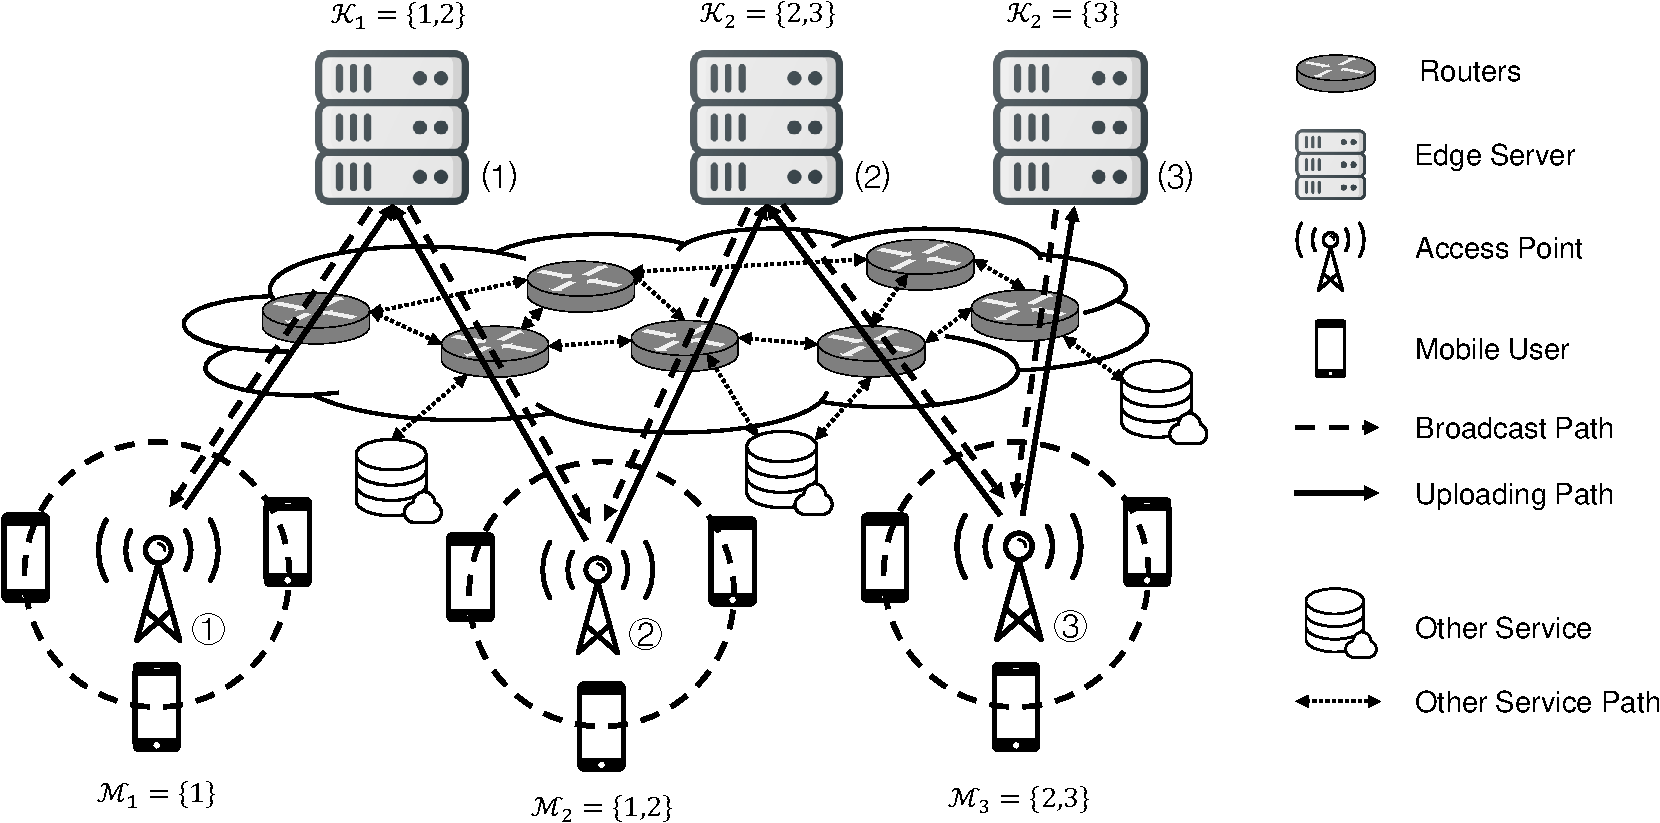
\includegraphics[width=0.60\textwidth]{system-model.pdf}
    \caption{The Illustration of System Model}
    \label{fig:system}
\end{figure*}

We consider an edge computing system with $K$ Access Points (APs) and $M$ edge servers, which are connected in a network as illustrated in Fig.\ref{fig:system}.
The sets of APs and edge servers are denoted as $\apSet \define \set{1,\dots,K}$ and $\esSet \define \set{1,\dots,M}$, respectively.
The communication latency among these APs and edge servers is random.
Without loss of generality, it is assumed that there are $J$ types of jobs computed in this system, which are denoted via the set $\mathcal{J} \define \set{1,\dots,J}$.
Each AP collects the computation jobs from the mobile users within its coverage, and makes decision on the processing edge servers for each job type.
It is assumed that the $k$-th AP only dispatches the computation jobs to the edge servers within a certain number of hops.
Let $\esSet_{k} \subseteq \esSet$ be the set of edge servers which can compute the jobs from the $k$-th AP, and $\apSet_{m}$ be the set of APs, which may upload jobs to the $m$-th edge server.
We refer to $\esSet_{k}$ as the \emph{candidate server set} of the $k$-th AP, and $\apSet_{m}$ as the \emph{potential AP set} of the $m$-th edge server ($\forall k\in\apSet, m\in\esSet$).
Different APs may have different candidate servers according to their locations in the network, as illustrated in Fig.\ref{fig:system}.
In this edge computing network, each AP and edge server periodically broadcast their state information (the state information is defined in the Section \ref{subsec:broadcast}), and one AP updates its strategy of job dispatching when receiving the broadcast state information.
In this paper, we shall optimize the job dispatching strategy distributed at APs with partially collected state information{, where both job uploading and state information broadcasting suffer from random transmission latency.}

%NOTE: [job space support and arrival process]
The time axis is organized by time slots.
The arrivals of the type-$j$ jobs at the $k$-th AP ($\forall k\in\apSet,j\in\jSpace$) in different time slots are assumed to be independent and identically distributed (i.i.d.) Bernoulli random variables, and the arrival probability is denoted as $\lambda_{k,j}$.
Let $A_{k,j}(t) \in \set{0,1}$ represents the event of job arrival, where $A_{k,j}(t)=1$ means one type-$j$ job arrives at the $k$-th AP in the $t$-th time slot, and $A_{k,j}(t)=0$ means otherwise.
Hence,
\begin{align}
    \Pr\{ A_{k,j}(t) = 1 \} = \lambda_{k,j}, \forall t,k\in\apSet,j\in\jSpace.
\end{align}

%NOTE: [uploading process]
Each AP immediately dispatches each type of received jobs to one edge server.
Different types of jobs may have different distributions of the input data size.
Moreover, due to the random traffic in the network, the job uploading from one AP to one edge server consumes a random number of time slots.
It is assumed that the random uploading latency are independent for each job.
Specifically, let $\mathbb{U}_{k,m,j}(\Xi)$ be the uploading latency distribution of the type-$j$ jobs from the $k$-th AP to the $m$-th edge server with support $\set{1, \dots, \Xi}$ ($\forall k\in\apSet, m\in\esSet, j\in\jSpace$), whose expectation is denoted as $u_{k,m,j}$.

%NOTE: [processing process]
There are $J$ parallel virtual machines (VMs) running on each edge server for processing the $J$ job types, respectively.
For each job type, the uploaded jobs are computed in a First-Come-First-Serve (FCFS) manner.
Hence, a processing queue with a maximum job number $L_{max}$ is established for each VM.
The arrival jobs will be discarded when the processing queue is full.
Furthermore, we adopt the \emph{unrelated machines assumption} as in \cite{tan-online}, and assume that the computation time of different job types on different edge servers follows independent memoryless geometric distribution 
\footnote{In this paper, we adopt the memoryless geometric distribution to simplify the elaboration of notations. In fact, the proposed algorithm can be easily extended to other distributions.}
with different expectations \cite{TOWC18-HuangKb}.
Let $\mathbb{G}(1/c_{m,j})$ be the distribution of the computation time slots for the type-$j$ jobs on the $m$-th edge server, where $\mathbb{G}$ denotes the geometric distribution, and $c_{m,j}$ is the expectation.
Let $f_{m,j}$ be its probability mass function (PMF), we have
\begin{align}
    f_{m,j}(x) \define (1-\frac{1}{c_{m,j}})^{x-1} \frac{1}{c_{m,j}}.
\end{align}
%----------------------------------------------------------------------------------------%

\subsection{Periodic Broadcast of State Information}
\label{subsec:broadcast}
In order to facilitate distributed dispatching for the APs, we refer to every $t_B$ time slots as a broadcast interval.
As illustrated in Fig.\ref{fig:brd-timeline}, at the beginning of each broadcast interval, the local state information (LSI) of APs and edge servers are broadcast, and each AP updates its strategy of job dispatching when {observing} the broadcast LSIs {from some APs and edge servers. As a remark notice that the observed LSI may be outdated due to transmission latency among APs and edge servers.}
The LSI at the APs and edge servers, global state information, and observed LSI at the APs are defined below.

%NOTE: State and Broadcast Information for AP
\begin{definition}[Local State Information of APs]
    Let $R^{(k)}_{m,j}(\xi,t,n) \in \set{0,1}$ be the indicator of the type-$j$ jobs at the $n$-th time slot of the $t$-th interval.
    Its value is $1$ when there is one job being uploaded from the $k$-th AP to the $m$-th server which has been delivered for $\xi$ time slots, and $0$ otherwise.
    Let $\omega_{k,j}(t)$ be the target processing edge server for the type-$j$ jobs of the $k$-th AP at the very beginning of the $t$-th broadcast interval, and $\omega_{k,j}(t+1)$ be the updated target processing edge server when the $k$-th AP observe a number of the broadcast LSIs of the $t$-th broadcast interval.
    The LSI of the $k$-th AP at the beginning of the $t$-th broadcast interval is defined as
    {\small
    \begin{align}
        \mathcal{R}_{k}(t) \define
        \Paren{
            \Brace{\vec{R}^{(k)}_{m,j}(t,0) \Big| \forall m\in\esSet,j\in\jSpace},
            \mathcal{A}_{k}(t)
        },
    \end{align}
    }
    where
    \begin{align}
        \vec{R}^{(k)}_{m,j}(t,0) \define \Paren{
            R^{(k)}_{m,j}(0,t,0), \dots, R^{(k)}_{m,j}(\Xi,t,0)
        },
    \end{align}
    and
    \begin{align}
        \mathcal{A}_{k}(t) &\define \Brace{\omega_{k,j}(t) \Big| \forall j\in\jSpace}
    \end{align}
    is referred as the dispatching actions of the $k$-th AP at the start of the $t$-th broadcast interval.
\end{definition}

%NOTE: State and Broadcast Information for Edge Server
\begin{definition}[Local State Information of Edge Servers]
    Let $Q_{m,j}({t,n})$ be the number of type-$j$ jobs on the $m$-th edge server at the $n$-th time slot of the $t$-th interval ($\forall m\in\esSet, j\in\jSpace$).
    The LSI of the $m$-th edge server at the $t$-th broadcast interval is defined as
    \begin{align}
        \mathcal{Q}_{m}(t) \define \Brace{
            Q_{m,j}(t, 0) \Big| \forall j\in\jSpace
        }.
    \end{align}
\end{definition}

\begin{definition}[Global State Information]
    The global state information (GSI) of the $t$-th broadcast interval is defined as the aggregation of the broadcast LSIs from all the APs and edge servers, i.e.,
    \begin{align}
        \Stat(t) \define
            \Paren{
                \Brace{\mathcal{R}_{k}(t) \Big| \forall k\in\apSet},
                \Brace{\mathcal{Q}_{m}(t) \Big| \forall m\in\esSet}
            }.
    \end{align}
\end{definition}

%NOTE: Conflict of AP set and partial information definition
As the APs and edge servers may reside in different locations of a MAN, the transmission latency of LSI is not negligible.
It might be inefficient for one AP (say the $k$-th AP) to collect the complete GSI before update the dispatching policy.
For example, the transmission latency of the LSI from the edge servers out of its \emph{candidate server set} $\esSet_{k}$ may be large, and some broadcast information may be discarded by the routers after a certain number of hops.
In this paper, we shall investigate the dispatching design based on the \emph{observed state information} at each AP.
Specifically, the \emph{conflict AP sets} and the \emph{observed state information} are defined below, respectively.
\begin{definition}[Conflict AP Set]
    The conflict AP set to the $k$-th AP consists of the neighboring APs who have direct impact on the queueing time of the jobs dispatched from the $k$-th AP, i.e.,
    \begin{align}
        \ccSet_{k} \define \bigcup_{m\in\esSet_{k}} \apSet_{m}.
    \end{align}
\end{definition}

\begin{definition}[Observed State Information]
    The observed state information (OSI) of the $k$-th AP ($\forall k\in\apSet$) at the $t$-th broadcast interval is defined as the aggregation of LSIs of the APs in {conflict AP set} and the edge servers in {candidate server set} of the $k$-th AP, i.e.,
    \begin{align}
        \Stat_{k}(t) &\define
        \Paren{
            \Brace{\mathcal{R}_{k'}(t) \Big| \forall k'\in\ccSet_{k}},
            \Brace{\mathcal{Q}_{m}(t) \Big| \forall m\in\esSet_{k}}
        }.
    \end{align}
    \label{def:OSI}
\end{definition}

\begin{figure*}[t]
    \centering
    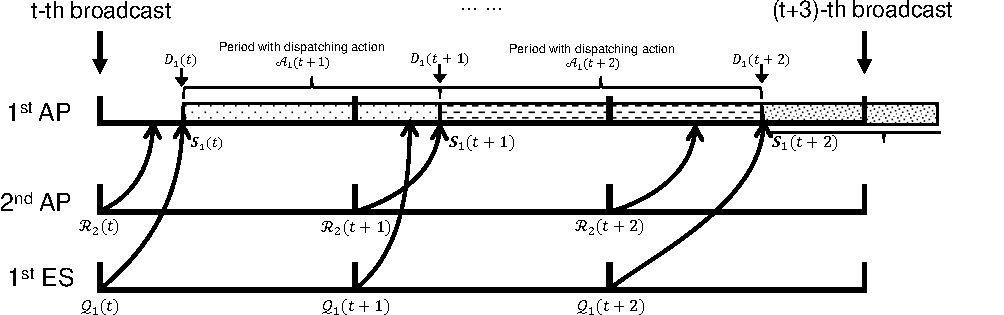
\includegraphics[width=0.60\textwidth]{brd-timeline.pdf}
    \caption{The timeline illustration of reception of OSI for the $1$-st AP where $2$-nd AP is in its \emph{conflict AP set} and $1$-st server is in its \emph{candidate server set}.}
    \label{fig:brd-timeline}
\end{figure*}

The $k$-th AP is able to collect its OSI at the $\mathcal{D}_{k}(t)$-th time slots of the $t$-th broadcast interval, where the \brlatency~$\mathcal{D}_{k}(t)$ is a random variable.
It is assumed that $\mathcal{D}_{k}(t)$ follows identical and independent distribution in different broadcast interval.
We refer to $\mathcal{D}_{k}(t)$ as the \brlatency~of the $k$-th AP at the $t$-th broadcast interval.
An example is given below to demonstrate how the \brlatency~affects the reception of OSI and the update of the dispatching strategy.

\begin{example}
    An example is illustrated in Fig.\ref{fig:brd-timeline}, where the $2$-nd AP and $1$-st server are in the \emph{conflict AP set} and \emph{candidate server set} of the $1$-st AP, respectively.
    At the beginning of the $t$-th broadcast interval, the dispatching actions $\mathcal{A}_{1}(t)$ is adopted by the $1$-st AP.
    Then after $\mathcal{D}_{1}(t)$ time slots, it updates the dispatching actions to $\mathcal{A}_{1}(t+1)$ based on the OSI.
    At the start of the $(t+1)$-th broadcast interval, it will firstly keep the previous actions, and then updates the actions immediately $\mathcal{D}_{1}(t+1)$ time slots later which is denotes as $\mathcal{A}(t+2)$.
    The signaling latency $\mathcal{D}_1(t)$ and $\mathcal{D}_1(t+1)$ can be different.
\end{example}

    \section{POMDP-based Problem Formulation}
\label{sec:formulation}
%----------------------------------------------------------------------------------------%
In this section, we formulate the optimization of job dispatching at all APs as a Markov decision process (MDP) problem.
Since each AP update the job dispatching actions according to OSI instead of GSI, the MDP problem is a partially observable MDP (POMDP).
Specifically, the individual dispatching policy of one AP, the system dispatching policy, and the cost function are first defined below.

\begin{definition}[Dispatching Policy]
    The individual policy of the $k$-th AP, denoted as $\Omega_{k}$ ($\forall k \in\apSet$), maps from its OSI $\Stat_{k}$ and its \brlatency~$\mathcal{D}_{k}$ to the dispatching action for each job type, i.e.,
    \begin{align}
        \Omega_{k} \Paren{ \Stat_{k}(t), \mathcal{D}_{k}(t) }
        &\define \mathcal{A}_{k}(t+1)
        \nonumber\\
        &= \Brace{
            \omega_{k,j}(t+1) \Big| \forall j\in\jSpace
        }.
        \label{def:action}
    \end{align}

    The aggregation of individual policy of all APs is referred to as the system dispatching policy $\Policy$.
    Thus,
    {
    \begin{align}
        \Policy\Paren{ \Stat(t), \Delay(t) } \define \Brace{
            \Omega_{1}(\Stat_{1}(t), \mathcal{D}_{1}(t)), \dots, \Omega_{K}(\Stat_{K}(t),\mathcal{D}_{K}(t))
        },
    \end{align}
    }
    where $\Delay(t) \define \set{ \mathcal{D}_{1}(t), \dots, \mathcal{D}_{K}(t) }$.
\end{definition}

According to the Little's law \cite{Little1961}, the average response time per job, counting the number of broadcast intervals from job arrival to the accomplishment of computation, is proportional to the number of jobs in the system, given the job arrival rates at all the APs.
Hence, we define the cost function per broadcast interval as follows.

\begin{definition}[Cost Function per Broadcast Interval]
    The cost function of the $t$-th broadcast interval with GSI $\Stat(t)$ is defined as
    {
    \begin{align}
        g\Paren{\Stat(t)} \define
            \sum_{m\in\esSet,j\in\jSpace}
            \Brace{&
                \sum_{k\in\apSet} \Inorm{\vec{R}^{(k)}_{m,j}(t,0)} + Q_{m,j}(t,0)
                + \beta \cdot I[Q_{m,j}(t,0)=L_{max}]
            },
    \end{align}
    }where $\Inorm{\vec{x}}$ denotes the $L^1$-norm of the vector $\vec{x}$, and $\beta$ is the weight of overflow penalty.
\end{definition}

Since the job dispatching in one broadcast interval will affect the GSI of the following broadcast intervals, we should consider the joint minimization of the costs of all the broadcast intervals.
Specifically, we consider the following discounted sum of the costs of all the broadcast intervals as the system objective.
\begin{align}
    &\bar{G}(\Stat, \Policy) \define
    \lim_{T \to \infty} \mathbb{E}^{\Policy}_{\set{\Stat(t)|\forall t}}
    \Bracket{
        \sum_{t=1}^{T} \gamma^{t-1} g\Paren{\Stat(t)} \Big| \Stat(1)
    },
\end{align}
where $\mathbb{E}^{\Policy}_{\set{\Stat(t)|\forall t}}[\cdot]$ denotes the expectation with respect to all possible system state in the future given scheduling policy $\Policy$, and $\gamma \in (0,1)$ is the discount factor.
Hence, the optimization of job dispatching policy can be formulated as the following minimization problem.
\begin{align}
    \textbf{P1:}~
    \min_{\Policy} \bar{G}(\Stat, \Policy).
\end{align}

If the GSI $\Stat(t)$ and \brlatency~$\Delay(t)$ are known to all the APs, the MDP in problem P1 can be solved via the following Bellman's equations as in \cite{sutton1998}.
{\small
\begin{align}
    &V\Paren{\Stat(t)} =g\Paren{\Stat(t)}
        + \gamma\mathbb{E}_{\Delay}\bigg\{
            \min_{\Policy(\Stat(t),\Delay(t))}
            \sum_{\Stat(t+1)} \Pr \Big\{ 
                \Stat(t+1) \Big| \Stat(t), \Policy(\Stat(t), \Delay(t)) \Big\} \cdot V\Big(\Stat(t+1)\Big)
            \bigg\},
    \label{eqn:sp_0}
\end{align}
}
where the value function $V(\Stat(t))$ of the optimal policy $\Policy^{*}$ (if GSI and \brlatency~are known to all the APs) is defined as follows.
\begin{align}
    &V\Paren{\Stat(t)} \define
    \lim_{T\to\infty} 
    \mathbb{E}^{\Policy^*}_{\set{\Stat(t)|\forall t}, \Delay} \Bracket{
        \sum_{t=1}^{T} \gamma^{t-1} g\Big( \Stat(t) \Big) \Big| \Stat(1)
    }.
    \label{eqn:val_f}
\end{align}
Moreover, the optimal policy $\Omega^{*}$ can be obtained by solving the right-hand-side (RHS) of the above Bellman's equations.

However, it is infeasible to solve the above Bellman's equations in our problem {and achieve the performance of $\Policy^*$ in our problem.}
This is because each AP (say the $k$-th AP) only has the knowledge of its own OSI $\Stat_{k}(t)$ and local \brlatency~$\mathcal{D}_{k}(t)$.
Thus, problem P1 is actually a POMDP.
The general solution of POMDP is of huge complexity {as all the historical system states should be involved in the current system state} \cite{IJCAI03-NairR,IJCAI99-BoutilierC}.
In this paper, we shall propose a novel low-complexity solution framework based on an analytical approximation of the value function $V(\cdot)$ and alternative actions update, where distributed job dispatching via the Bellman's equations becomes feasible even with OSI and local signaling latency.
%----------------------------------------------------------------------------------------%


    \section{Distributed Algorithm with Partial Information}
\label{sec:algorithm}

In this section, we shall introduce a novel approximation method to decouple the centralized optimization on the RHS of the Bellman's equations to each AP for arbitrary system state.
Specifically, the decoupling can be achieved via the following two steps:
\begin{enumerate}
    \item We first introduce a baseline policy, use its value function to approximate the value function of the optimal policy $\Policy^*$, and derive the analytical expression of the approximate value function in Section \ref{subsec:baseline}.
    \item Based on the approximate value function, an alternative action update algorithm, where a subset of APs are selected to update their dispatching action distributed in each broadcast interval, is proposed to solve the RHs of the Bellman's equation in equation (\ref{eqn:sp_0}) in Section \ref{subsec:ap_alg}.
    Moreover, the analytical performance bound is also derived in Section \ref{subsec:analysis}.
\end{enumerate}
{As a remark notice that solving the value function and then the RHS of the Bellman's equations are the two standard steps to solve an MDP problem with complete knowledge on system state.
These approaches cannot be used for POMDP.
In our proposed approximate solution framework, however, we follow a similar two-step procedure but with novel techniques to solve the POMDP problem in P1: (1) find approximate value function, instead of solving the accurate value function V; (2) use alternative method to optimize the RHS of the Bellman's equation gradually, instead of simultaneous action optimization at all APs.}

\subsection{Baseline Policy and Approximate Value Function}
\label{subsec:baseline}
To alleviate the curse of dimensionality, we first use the baseline policy with fixed dispatching action to approximate value function at the RHS of the Bellman's equations in equation (\ref{eqn:val_f}).
Specifically, the baseline policy is elaborated below.

\begin{policy}[Baseline Policy]
    In the baseline policy $\Baseline$, each AP fixes the target processing edge server for each job type as the previous broadcast interval. Specifically, at the $t$-th broadcast interval,
    \begin{align}
        \Baseline(\Stat(t)) &\define \Bracket{ \Pi_{1}(\Stat_{1}(t)), \dots, \Pi_{K}(\Stat_{K}(t)) },
    \end{align}
    where 
    \begin{align}
        \Pi_{k}(\Stat_{k}(t)) &\define
        \hat{\mathcal{A}}_{k}(t)
        \nonumber\\
        &= \Brace{
            \omega_{k,j}(t) \Big| \forall j\in\jSpace
        }, \forall k\in\apSet.
    \end{align}
\end{policy}

Let $W_{\Baseline}(\cdot)$ be the value function of the baseline policy, we shall approximate the value function of the optimal policy $V(\cdot)$ via $W_{\Baseline}$, i.e.,
{
\begin{align}
    V\Paren{\Stat(t+1)} &\approx W_{\Baseline}\Paren{\Stat(t+1)}
    \nonumber\\
    &= \sum_{m\in\esSet,j\in\jSpace}\Brace{
        \sum_{k\in\apSet} \tilde{W}^{\AP}_{k,m,j}(\Stat(t+1))
        +\tilde{W}^{\ES}_{m,j}(\Stat(t+1))
    },
\end{align}
}
where $\tilde{W}^{\AP}_{k,m,j}(\Stat(t+1))$ denotes the cost raised by the type-$j$ jobs which are being transmitted from the $k$-th AP to the $m$-th edge server with the baseline policy $\Baseline$ and initial system state $\Stat(t+1)$, and $\tilde{W}^{\ES}_{m,j}(\Stat(t+1))$ denotes the cost raised by the type-$j$ jobs on the $m$-th server.
Their definitions are given below.
{
\begin{align}
    \tilde{W}^{\AP}_{k,m,j} \Paren{\Stat(t+1)} &\define
        \sum_{i=0}^{\infty} \gamma^{i+1} \mathbb{E}^{\Baseline}\Bracket{
            \Inorm{\vec{R}^{(k)}_{m,j}(t+i+1)}
        },
    \\    
    \tilde{W}^{\ES}_{m,j} \Paren{\Stat(t+1)} &\define
        \sum_{i=0}^{\infty} \gamma^{i+1} \mathbb{E}^{\Baseline}\Bracket{
            Q_{m,j}(t+i+1) + \beta I[Q_{m,j}(t+i+1) = L_{max}]
        }.
\end{align}
}

Moreover, the explicit expressions of $\tilde{W}^{\AP}_{k,m,j}(\Stat(t+1))$ and $\tilde{W}^{\ES}_{m,j}(\Stat(t+1))$ are derived in the following lemmas, respectively.

\begin{lemma}[Analytical Expression of $\tilde{W}^{\AP}_{k,m,j}$]
    \label{lemma:w_ap}
    \begin{align}
        &\tilde{W}^{\AP}_{k,m,j}\Paren{\Stat(t+1)} =
        \Inorm{
            \vecG{\Theta}^{(k, \Baseline)}_{m,j}(t+1) \times
            \Bracket{
                \mat{I} - \gamma \Gamma^{(k)}_{m,j}
            }^{-1}
        },
        \label{w_ap}
    \end{align}
    where $\mat{I}$ is the identity matrix, and $\vecG{\Theta}^{(k, \Baseline)}_{m,j}(t)$ and $\Gamma^{(k)}_{m,j}$ are defined below.
    \begin{itemize}
        \item {$\vecG{\Theta}^{(k,\Baseline)}_{m,j}(t) \define \Bracket{
            \theta^{(k,\Baseline)}_{m,j}(0,t),
            \theta^{(k,\Baseline)}_{m,j}(1,t),
            \dots,
            \theta^{(k,\Baseline)}_{m,j}(\Xi,t)
            }$},
        where 
        \begin{align}
            \theta^{(k)}_{m,j}(\xi,t) \define 
            \begin{cases}
                \lambda_{k,j} I[\omega_{k,j}(t)=m], & \xi=0
                \\
                \Pr\{R^{(k)}_{m,j}(\xi,t,0) = 1\}, & \text{otherwise}
            \end{cases}
        \end{align}
        \item $\Gamma^{(k)}_{m,j} \in \mathbb{R}^{(\Xi+1)\times(\Xi+1)}$ denotes the transition matrix.
    \end{itemize}
\end{lemma}
\begin{proof}
    \comments{The proof is removed which will be showed in the conference version.}
\end{proof}

\begin{lemma}[Analytical Expression of $\tilde{W}^{\ES}_{m,j}$]
    \label{lemma:w_es}
    {
    \begin{align}
        &\tilde{W}^{\ES}_{m,j}\Paren{\Stat(t+1)}
    = \sum_{i=0,\dots,\frac{\Xi}{T}} \gamma^{i} \mathbb{E}^{\Baseline}[ Q_{m,j}({t+i+1}) | \Stat(t+i)]
    \nonumber\\
    &~~~~~~~~~~~~+ \gamma^{\frac{\Xi}{T}} 
    \vecG{\nu}({t+\frac{\Xi}{T}+1})
    \Paren{
        \mat{I} - \gamma \mat{P}^{\Baseline}_{m,j}(t)
    }^{-1} \vec{g}',
        \label{w_es}
    \end{align}   
    }
    where $\vecG{\nu}_{m,j}(t)$, $\mat{P}_{m,j}(\beta_{m,j}(t))$, $\beta_{m,j}(t)$ and $\vec{g}$ are defined below.
    \begin{itemize}
        \item {
        $\vecG{\nu}_{m,j}(t) \define [\Pr\{Q_{m,j}(t)=0\}, \dots, \Pr\{Q_{m,j}(t)=L_{max}\}]$
        }.
        \item $\vec{g} \in \mathbb{R}^{(L_{max}+1) \times 1}$, and its $i$-th entry is
        \begin{align}
            [\vec{g}]_{i} \define 
            \begin{cases}
                i, & i=0,1,\dots,L_{max}-1
                \\
                L_{max}+\beta, & \text{otherwise}
            \end{cases}.
            \label{eqn:g_vec}
        \end{align}
        % \item The expression of $\mathbb{E}^{\Baseline}[ Q_{m,j}({t+i+1}) | \Stat(t+i)]$ is elaborated.
        \item $\mat{P}^{\Baseline}_{m,j}(t) \in \mathbb{R}^{(L_{max}+1) \times (L_{max}+1)}$ denotes the transition matrix under baseline policy $\Baseline$.
    \end{itemize}   
\end{lemma}
\begin{proof}
    \comments{The proof is removed which will be showed in the conference version.}
\end{proof}

\subsection{Distributed Action Update}
\label{subsec:ap_alg}
Although the optimal value function has been approximated via the baseline policy in the previous part, it is still infeasible for all the APs to solve the RHS of the Bellman's equations in a distributed manner with OSI and local \brlatency~only.
This is because the evaluation of equation (\ref{w_ap}) and (\ref{w_es}) requires the knowledge of GSI and \brlatency~at all APs.
Instead, it is feasible for part of APs to update their dispatching actions distributed and achieve a better performance compared with baseline policy.
Hence, we first define the following sequence of AP subsets, where each subset are selected to update dispatching actions periodically.
\begin{definition}[Subsets of Periodic Actions Update]
    Let $\mathcal{Y}_{1}, \dots, \mathcal{Y}_{N} \subseteq \ccSet$ be a sequence of subset, where each subset satisfies the following constraints
    \begin{align}
        &\bigcup_{n=0,\dots,N-1} \mathcal{Y}_{n} = \apSet
        \\
        \esSet_{y} \cap \esSet_{y'} &=\emptyset, y' \neq y~(\forall y',y \in \mathcal{Y}_{n}).
    \end{align}
\end{definition}
For example, as illustrated in Fig.\ref{fig:system}, the AP set $\apSet$ could be decomposed of two subsets as $\set{1,3}$ and $\set{2}$.
At the $t$-th broadcast interval, the APs in the subset indexed with $n \define t \pmod{N}$ update their dispatching actions, while the other APs keep the same dispatching actions as the previous broadcast interval.
Hence, let 
\begin{align}
    \tilde{\mathcal{A}}_{y}(t) \define \Brace{\tilde{\omega}_{y,j}(t)\in \esSet_{y} \Big| \forall j\in\jSpace}
\end{align}
and 
\begin{align}
    \tilde{\mathcal{A}}(t) \define \Brace{\tilde{\mathcal{A}}_{y}(t) \Big| \forall y\in\mathcal{Y}_{n} }
\end{align}
be the aggregation of dispatching actions for the $y$-th AP and the APs in the subset $\mathcal{Y}_{n}$, respectively. Let
\begin{align}
    \hat{\mathcal{A}}(t) \define \Brace{\omega_{y,j}(t) \Big| \forall y\notin\mathcal{Y}_{n}, j\in\jSpace}
\end{align}
be the aggregation of dispatching actions of the rest APs, which are the same as the previous broadcast interval.
At the $t$-th broadcast interval, the optimization of $\tilde{\mathcal{A}}_{y}(t)$ ($\forall y\in\mathcal{Y}_{n}$) at the RHS of the Bellman's equations can be rewritten as the following problem.
{
\begin{align}
    \textbf{P2:}~
    \min_{ \tilde{\mathcal{A}}(t) }
    &\sum_{\Stat(t+1)} \Pr\Brace{
        \Stat(t+1) \Big| \Stat(t), \tilde{\mathcal{A}}(t), \hat{\mathcal{A}}(t)
    } \cdot W_{\Baseline}\Paren{\Stat(t+1)},
\end{align}
}

Moreover, we have the following conclusion on the decomposition of P2.
\begin{lemma}[]
    The optimization problem in P2 can be equivalently decoupled into local optimization problems at APs.
    Specifically, the local optimization at the $y$-th AP ($\forall y\in\mathcal{Y}_{n}$) can be written as
    \begin{align}
        &\textbf{P3:}~
        \min_{ \tilde{\mathcal{A}}_{y}(t) }
        \mathbb{E}_{\set{ \Stat_{y}(t+1)|\Stat_{y}(t), \tilde{\mathcal{A}}_{y}(t) }}
        \nonumber\\
        &~~~~\sum_{j\in\jSpace,m\in\esSet_{y}} \Brace{
            \tilde{W}^{\AP}_{y,m,j}\Paren{\Stat_{y}(t+1)}
            +\tilde{W}^{\ES}_{m,j}\Paren{\Stat_{y}(t+1)}
        }.
        \label{eqn:partial}
    \end{align} 
    \label{lemma:w_partial}
\end{lemma}
\begin{proof}
    At the $t$-th broadcast interval, the $y$-th AP in the subset $\mathcal{Y}_{n}$ updates its dispatching actions, which could only affect the future cost raised on itself and its corresponding \emph{candidate server set}, i.e., the part of its OSI.
    Hence, it's obvious that the expression of equation (\ref{w_ap}) and equation (\ref{w_es}) on the RHS of the Bellman's equations could be reduced into the form based only on the OSI of the $y$-th AP ($\forall y\in\mathcal{Y}_{n}$) as illustrated in equation (\ref{eqn:partial}).
\end{proof}

The optimization of $\tilde{\mathcal{A}}_{y}(t)$ for the $y$-th AP ($\forall y\in\mathcal{Y}_{n}$) in P3 could be achieved via searching all the edge servers in $\esSet_{y}$, whose computational complexity is $O(JMK)$ per AP.
As a result, the overall algorithm of job dispatching is elaborated in Algorithm \ref{alg_1}.
\begin{algorithm}[ht]
    \caption{Online Alternative Actions Update Algorithm}\label{alg_1}
    \DontPrintSemicolon % Some LaTeX compilers require you to use \dontprintsemicolon instead
    % \KwIn{$\Stat(t), \Delay(t)$}
    % \KwOut{$\tilde{\mathcal{A}}(t)$}
    Initialize $\tilde{\mathcal{A}}(0),\hat{\mathcal{A}}(0)$ with heuristic dispatching actions.\;
    \For{$t=0,1,2,\dots$}{
        \tcc{Get the index of the subset to update at $t$.}
        $n \gets t \pmod{N}$\;
        \tcc{Parallelly update the actions of APs in the subset $\mathcal{Y}_{n}$.}
        \ForPar{$y \in \mathcal{Y}_{n}$}{
            \tcc{Each AP observes its LSI asynchronously.}
            The $y$-th AP observes $\Stat_{y}(t)$ after $\mathcal{D}_{y}(t)$.\;
            \tcc{Then update actions by solving P3.}
            $\tilde{\mathcal{A}}_{y}(t+1) \gets$ solving P3 with $\Stat_{y}(t), \mathcal{D}_{y}(t)$\;
        }
        \tcc{The other APs fix the actions as the previous interval.}
        \ForPar{$y \not\in \mathcal{Y}_{n}$}{
            \eIf{$y\in\mathcal{Y}_{n-1}$}{
                $\hat{\mathcal{A}}_{y}(t+1) \gets \tilde{\mathcal{A}}_{y}(t)$
            }
            {
                $\hat{\mathcal{A}}_{y}(t+1) \gets \hat{\mathcal{A}}_{y}(t)$
            }
        }
        % \Return $\tilde{\mathcal{A}}(t+1)$\;
    }
\end{algorithm}

As a remark notice that Algorithm \ref{alg_1} leads to a time-variant policy, which is referred as the proposed policy $\tilde{\Policy}$.
At the $t$-th broadcast interval, the dispatching actions is given by
\begin{align}
    \tilde{\Policy}(\Stat(t), t) \define \tilde{\mathcal{A}}(t) \cup \hat{\mathcal{A}}(t).
\end{align}
This is because we choose different AP subset to update dispatching actions.
Since the AP subsets are selected periodically, we have $\tilde{\Policy}(\Stat, t) = \tilde{\Policy}(\Stat, t+N), \forall \Stat,t$.

\subsection{{Theoretical Analysis}}
\label{subsec:analysis}
Finally, we have the following conclusion on the performance of the above proposed algorithm.
\begin{lemma}[Analytical Cost Upper Bound]
    \label{lemma:bound}
    Let $W_{\tilde{\Policy}}(\cdot)$ be the value function of the policy $\tilde{\Omega}$
    \begin{align}
        W_{\tilde{\Policy}}(\Stat) \define
        \sum_{t'=1}^{\infty} \gamma^{t'-1} \mathbb{E}^{ \tilde{\Policy} } \Bracket{
            g\Paren{\Stat(t'), \tilde{\Policy}(\Stat(t'),t')} \Big| \Stat(1)=\Stat
        },
    \end{align}
    we have
    \begin{align}
        V_{\Policy^*}(\Stat)
        \leq W_{\tilde{\Policy}}(\Stat)
        \leq W_{\Baseline}(\Stat),
        \forall \Stat.
    \end{align}
\end{lemma}
\begin{proof}
    \comments{The proof is removed which will be showed in the conference version.}
\end{proof}
Therefore, the average system cost of the proposed algorithm is upper bounded by $W_{\Baseline}(\Stat)$ ($\forall \Stat$) which means it is always better than the baseline policy. 
% The worst case could be upper bounded.
%----------------------------------------------------------------------------------------%
%----------------------------------------------------------------------------------------%
    \section{Performance Evaluation}
\label{sec:evaluation}
In this section, we evaluate the performance of the proposed low-complexity dispatching policy $\tilde{\Policy}$ by numerical simulations.
The experiment setup and performance benchmarks are elaborated in Section \ref{subsec:setup}.
The simulation results are illustrated in Section \ref{subsec:basic}.
The sensitivity study on parameters is also applied to provide some insights on the robustness of the proposed policy in Section \ref{subsec:advance}.

\subsection{Experiment Setup}
\label{subsec:setup}
In the simulation, there are $K=5$ APs, $M=3$ edge servers and $J=5$ types of jobs in the system.
The edge servers are all fully-accessible to all the APs, i.e., $\esSet_{k}=\esSet$ ($\forall k\in\apSet$).

The time slot duration is 50 milliseconds and one broadcast interval consists of $t_{B}=20$ time slots, i.e., its duration is $1$ second.
The \brlatency~is a discrete random variable with an integer support from $10$ to $16$ time slots.
The maximum uploading latency is $3$ seconds, i.e., $\Xi = 3t_B$, and the distribution of $\mathbb{U}_{k,m,j}(\Xi)$ ($\forall k\in\apSet, m\in\esSet_{k}, j\in\jSpace$) is arbitrarily generated within the support $\set{0, 1, \dots, \Xi}$.
The expected computation time $c_{m,j}$ ($\forall m\in\esSet, j\in\jSpace$) is an integer uniformly generated in the range $[30,50]$ (with the unit of time slot) in each figure.

Each queue for VMs on edge server is with maximum queue length $L_{max}=20$, i.e., there would be at most $100$ jobs on one edge server.
The arrival rate in each time slot is uniformly generated from the range $[0.02, 0.03]$ for each job type at each AP in each figure.
The discount factor $\gamma$ is $0.95$ and the penalty weight $\beta$ is $20$.
% The arrival rate is taken as small probability with enough APs in the system, and correspondingly enough edge servers for the processing.

%-----------------------------------------------------------------------%
\begin{figure}[ht]                                                      %
    \centering                                                          %
    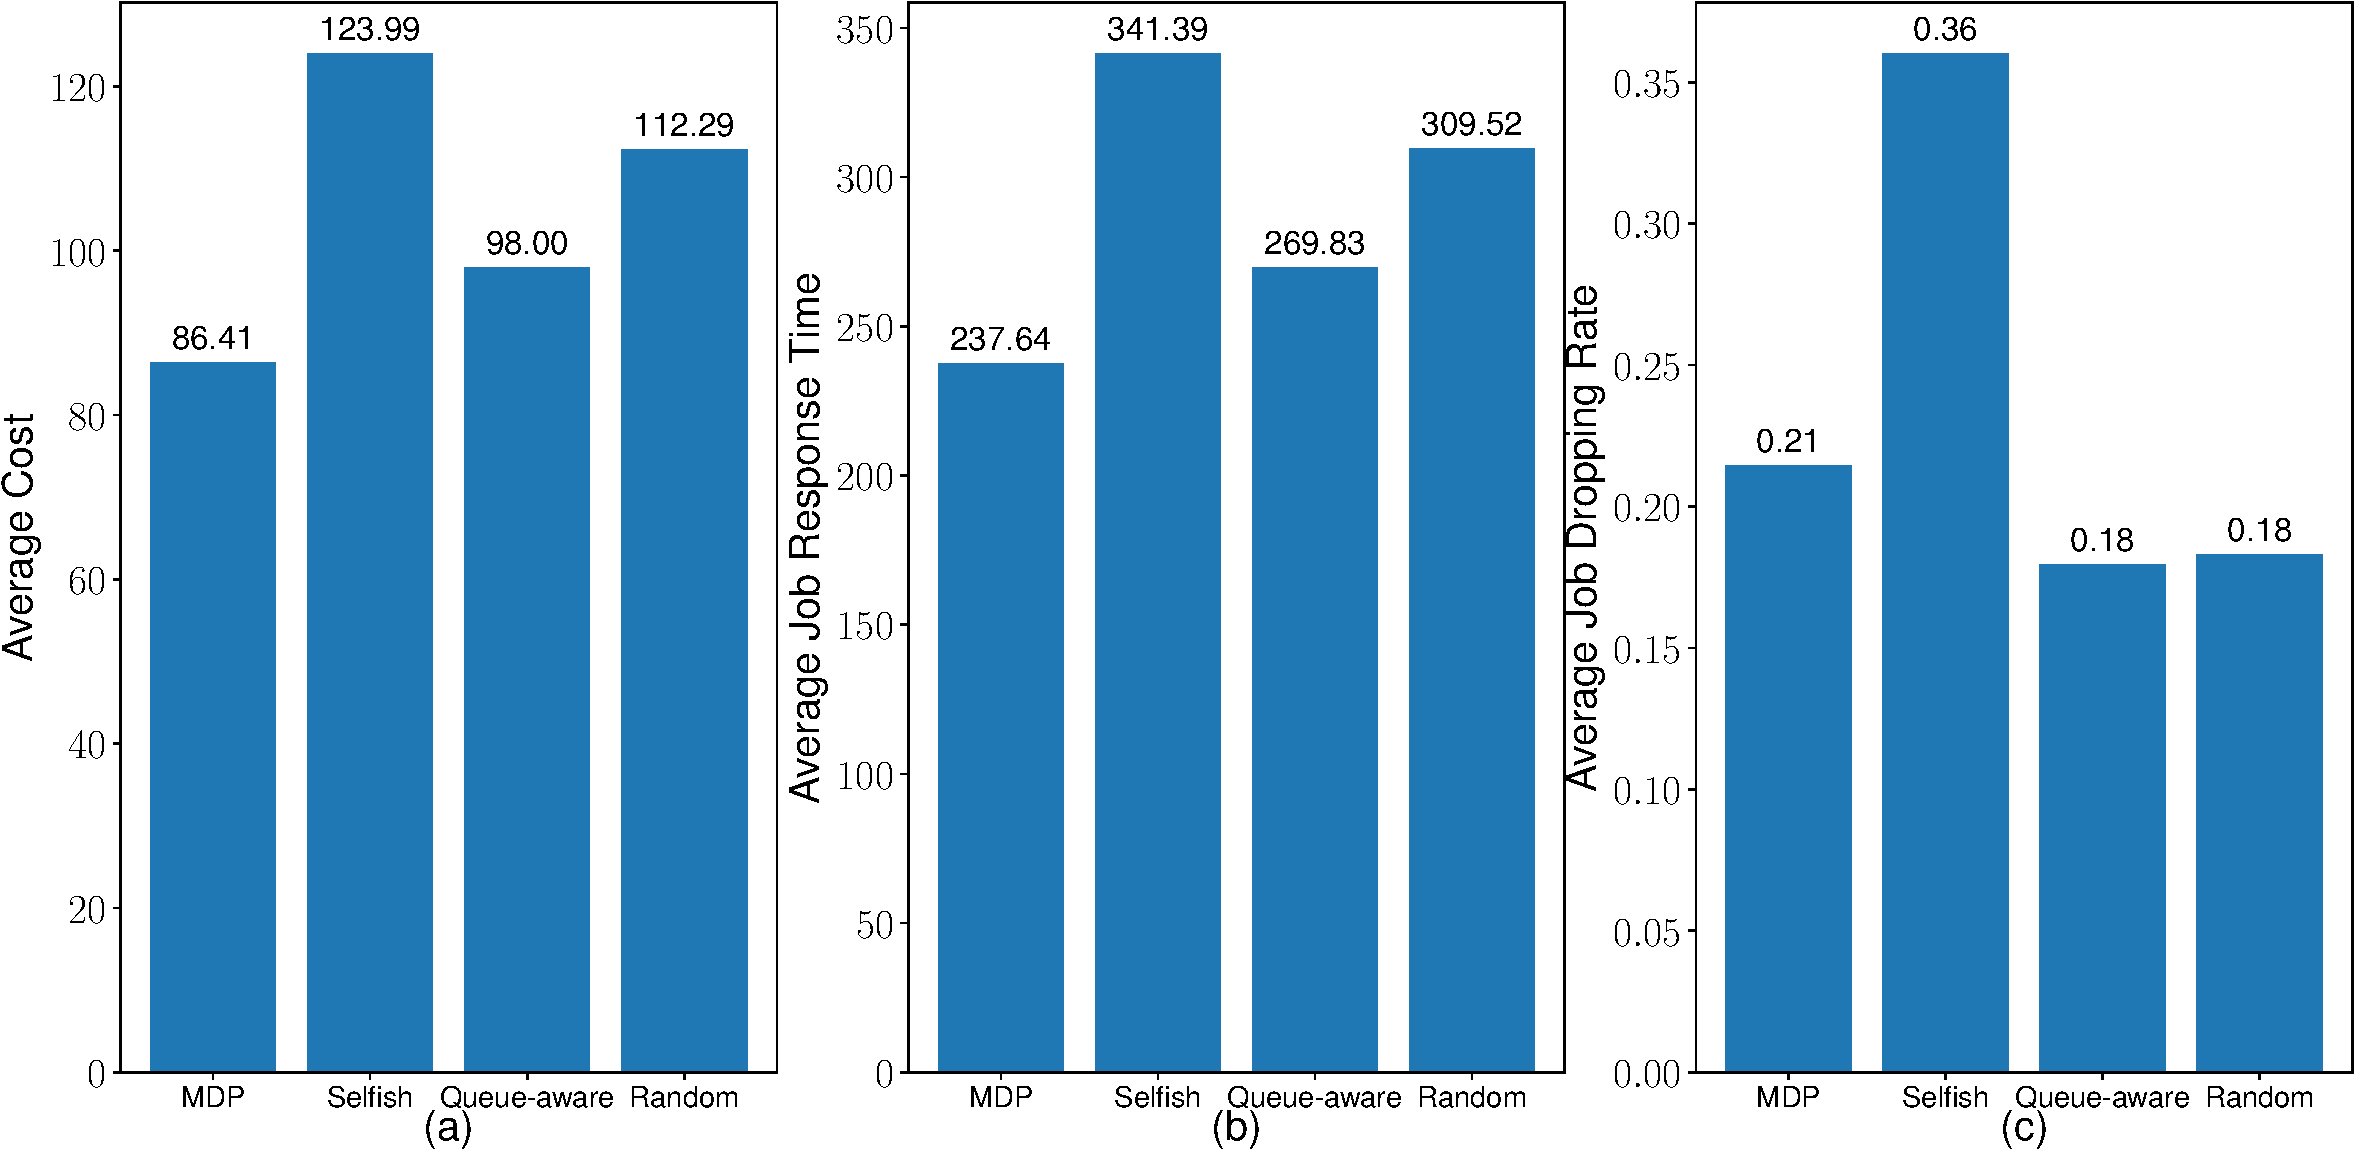
\includegraphics[width=0.85\textwidth]{41122-bar-graph-alter.pdf}   %
    \caption{Illustration of performance metrics comparison with benchmarks.}
    \label{fig:bar_plot}                                                %
\end{figure}                                                            %
%-----------------------------------------------------------------------%

%NOTE: Benchmark Elaboration
We compare the proposed MDP policy with other three benchmarks which are listed as follows.
\begin{itemize}
    \item \textbf{Random Dispatching Policy}:
            Randomly choose a dispatching edge server in each time slot; 
    \item \textbf{Selfish Policy}:
            Always choose the edge server with the minimum sum of the expected uploading time and processing time;
    \item \textbf{Queue-aware Policy}:
            Always choose the edge server with the minimum sum of expected uploading time, processing time and queueing time based on the observation of outdated queue states.
\end{itemize}
Moreover, we choose the Selfish Policy as the initial dispatching action for our proposed algorithm (Algorithm \ref{alg_1}).
%NOTE: Basic Performance
\subsection{Performance Analysis}
\label{subsec:basic}
As illustrated in Fig.\ref{fig:bar_plot}(a), the proposed algorithm (MDP Policy) outperforms all the benchmarks in the average system cost.
Moreover, the Queue-aware Policy has better performance than the other benchmarks due to its capability of adapting dispatching action according to the outdated observation of queueing state.
More insights on the performance comparison are provided in Fig.\ref{fig:bar_plot}(b) and (c).
In the former figure, the average job response times, measuring the average number of broadcast intervals from job's arrival at one AP to the completeness of computation at one edge server, are compared.
It can be observed that the proposed policy still outperforms all the benchmarks.
In Fig.\ref{fig:bar_plot}(c), the job dropping rates, measuring the ratio of jobs dropped by edge servers due to queue overflow, are also compared.
It is shown that the proposed policy can process the approximately the same number of jobs as Queue-aware Policy and Random Policy, while with the minimum average cost and job response time.
Finally, an realization of job dispatching is illustrated in Fig.\ref{fig:general_timeline}, where the number of jobs in the system is plot versus the index of broadcast interval.
It can be observed that the proposed policy manage to keep the number of jobs in lower level, compared with the benchmarks.
This demonstrates its high dispatching efficiency.

%-----------------------------------------------------------------------------------------------%
\begin{figure}[ht!]                                                                             %
    \centering                                                                                  %
    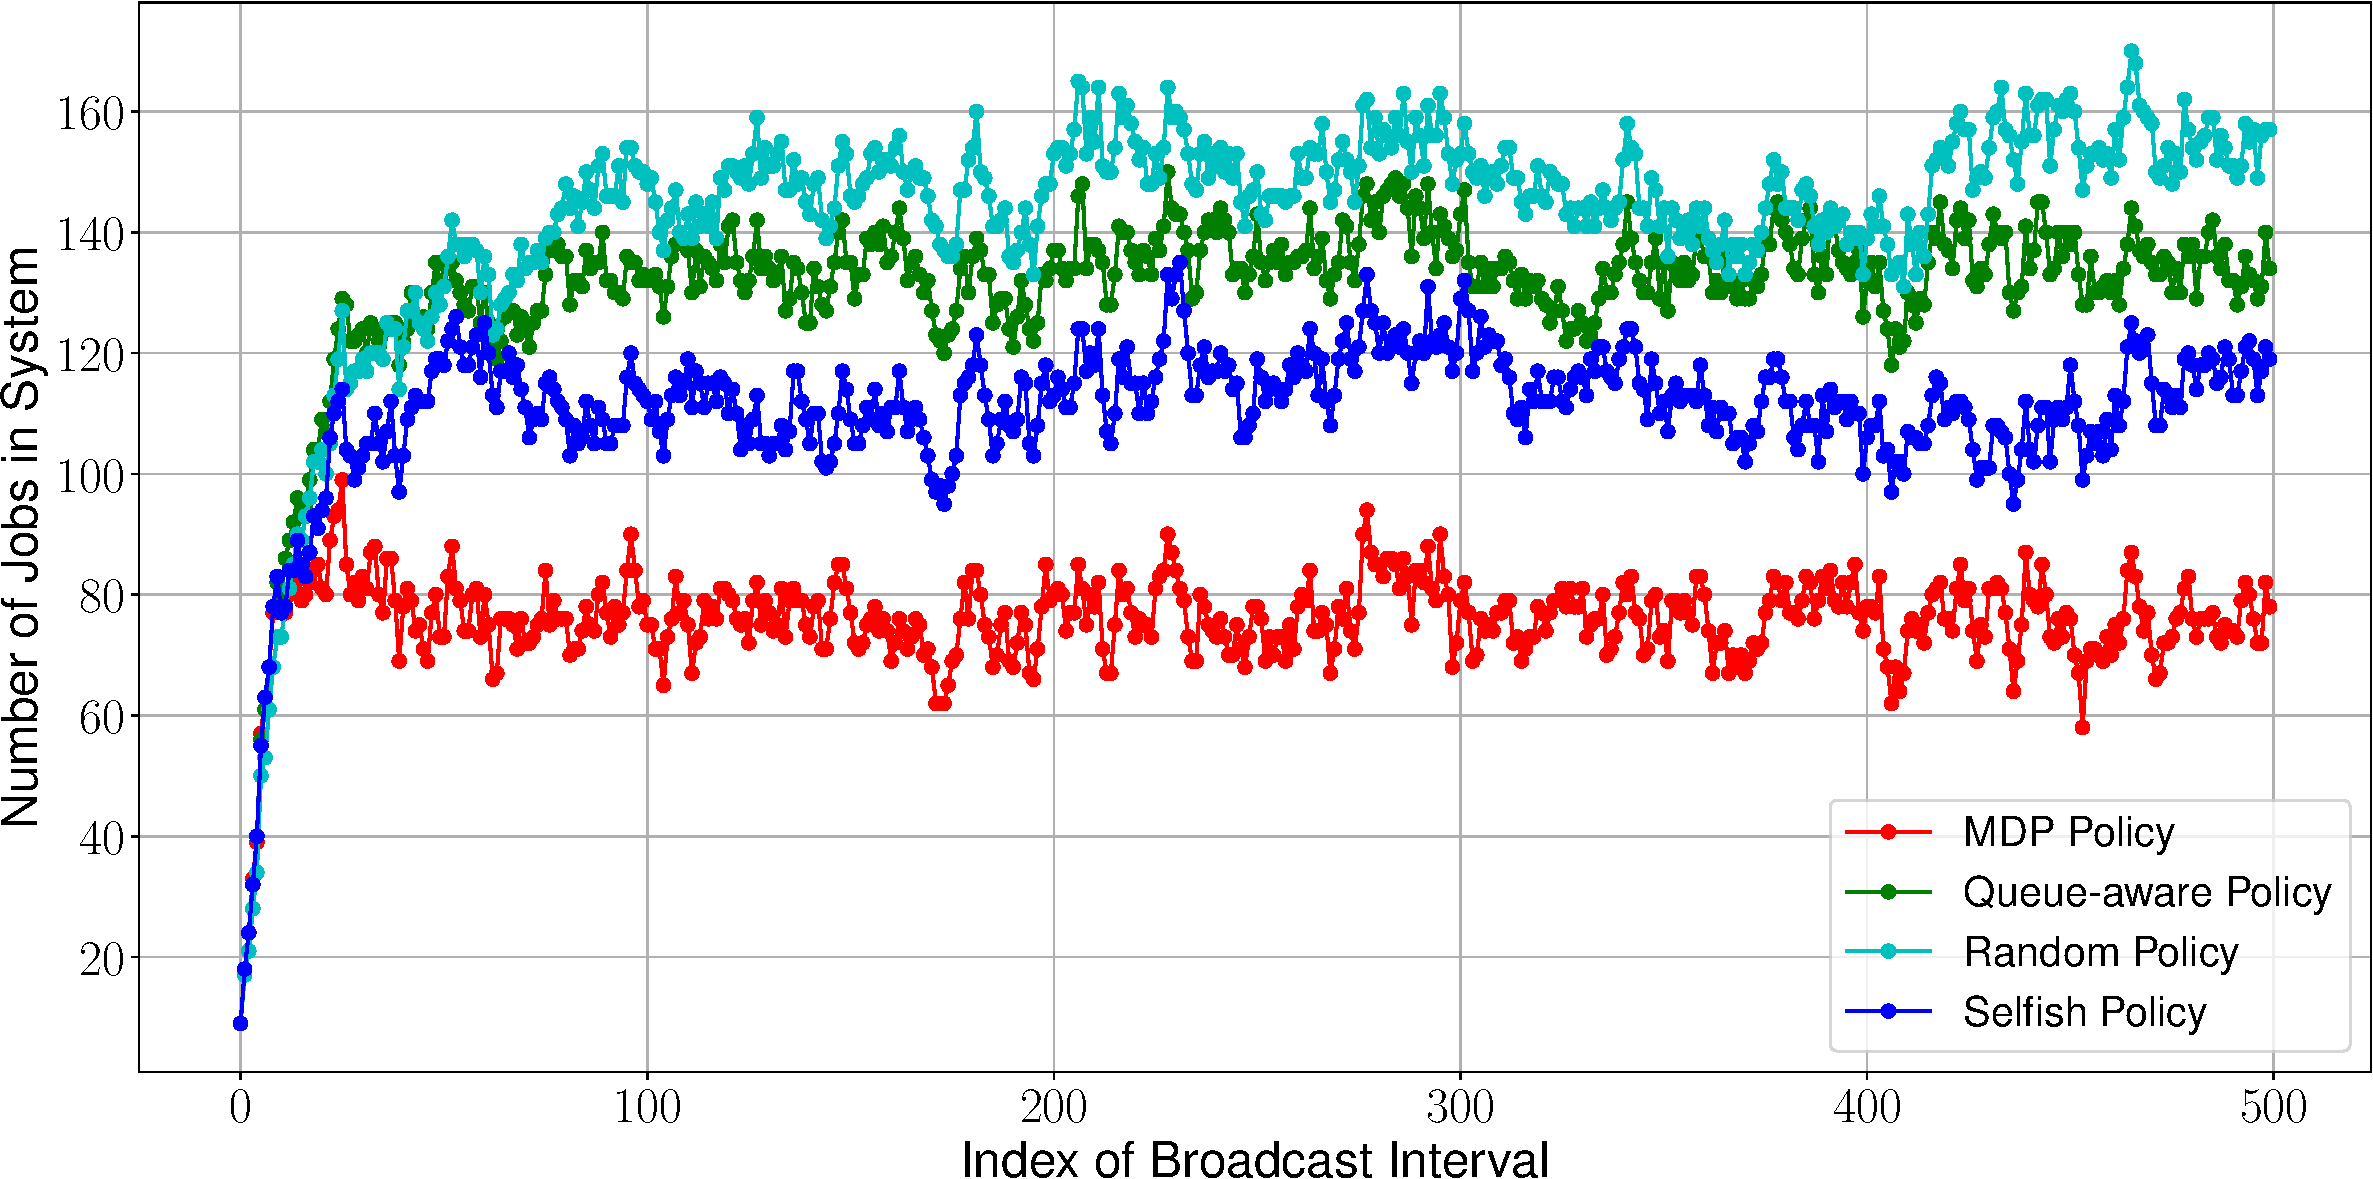
\includegraphics[width=0.85\textwidth]{41122-timeline-number-alter.pdf}                     %
    \caption{Illustration of number of jobs on all the APs and edge servers versus index of broadcast interval.}
    \label{fig:general_timeline}                                                                %
\end{figure}                                                                                    %
%-----------------------------------------------------------------------------------------------%

\subsection{Sensitivity Study}
\label{subsec:advance}  

%FIXME: replace the graphs
%-----------------------------------------------------------------------------------%
\begin{figure*}[ht!]                                                                %
    \centering                                                                      %
    \begin{tabular}{ccc}                                                            %
        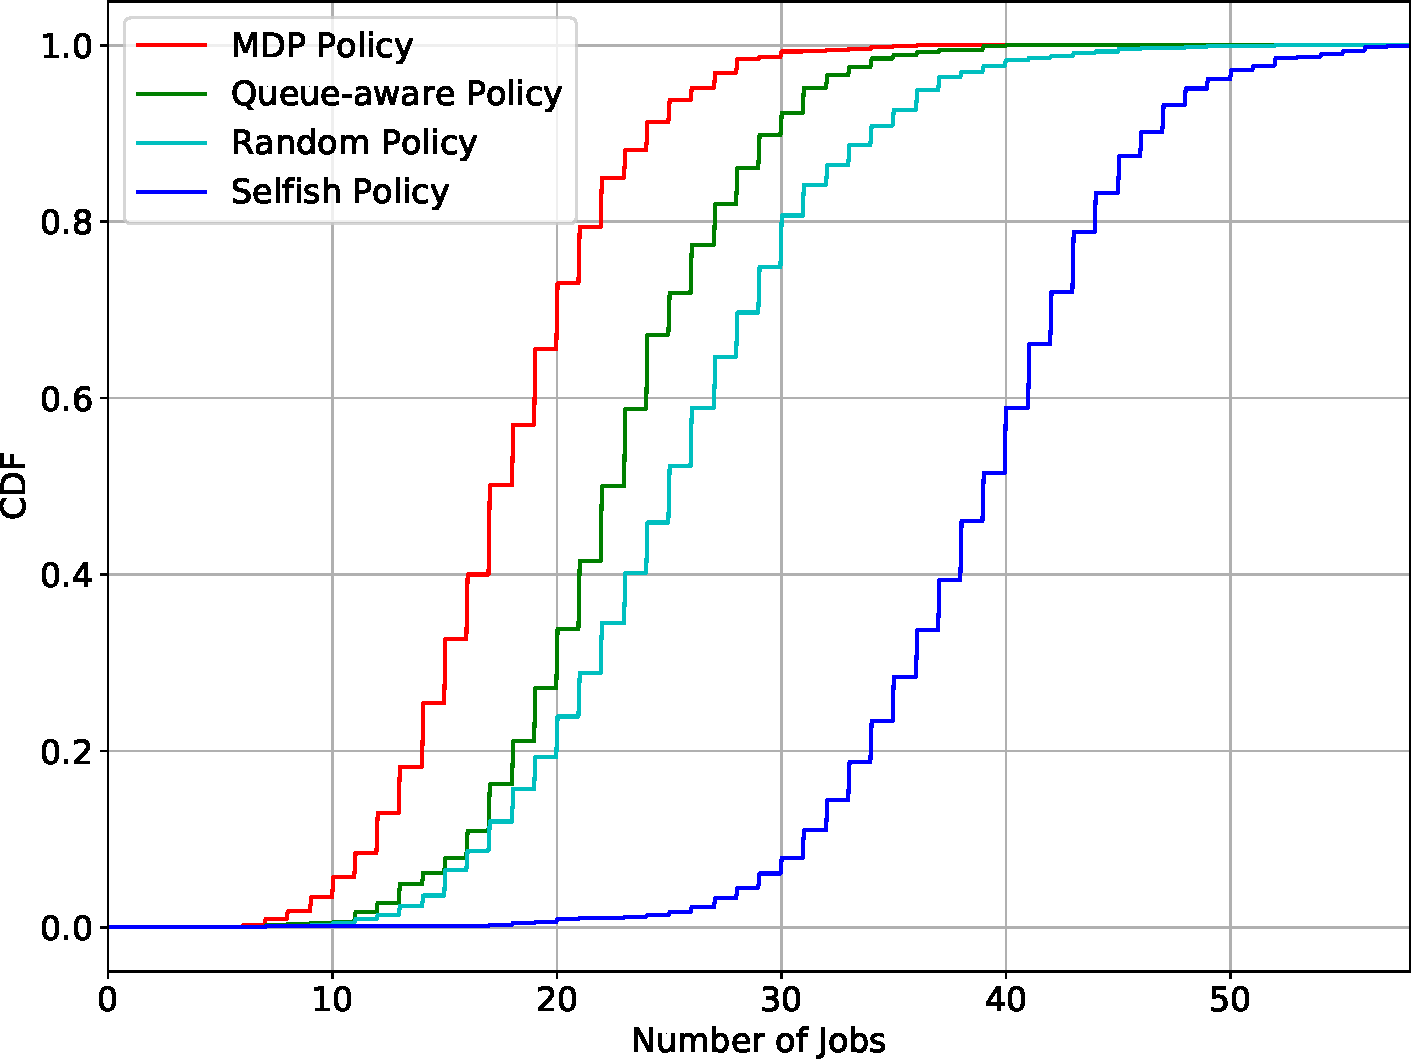
\includegraphics[width=0.30\textwidth]{LowPressure-d0.pdf}&                 %
        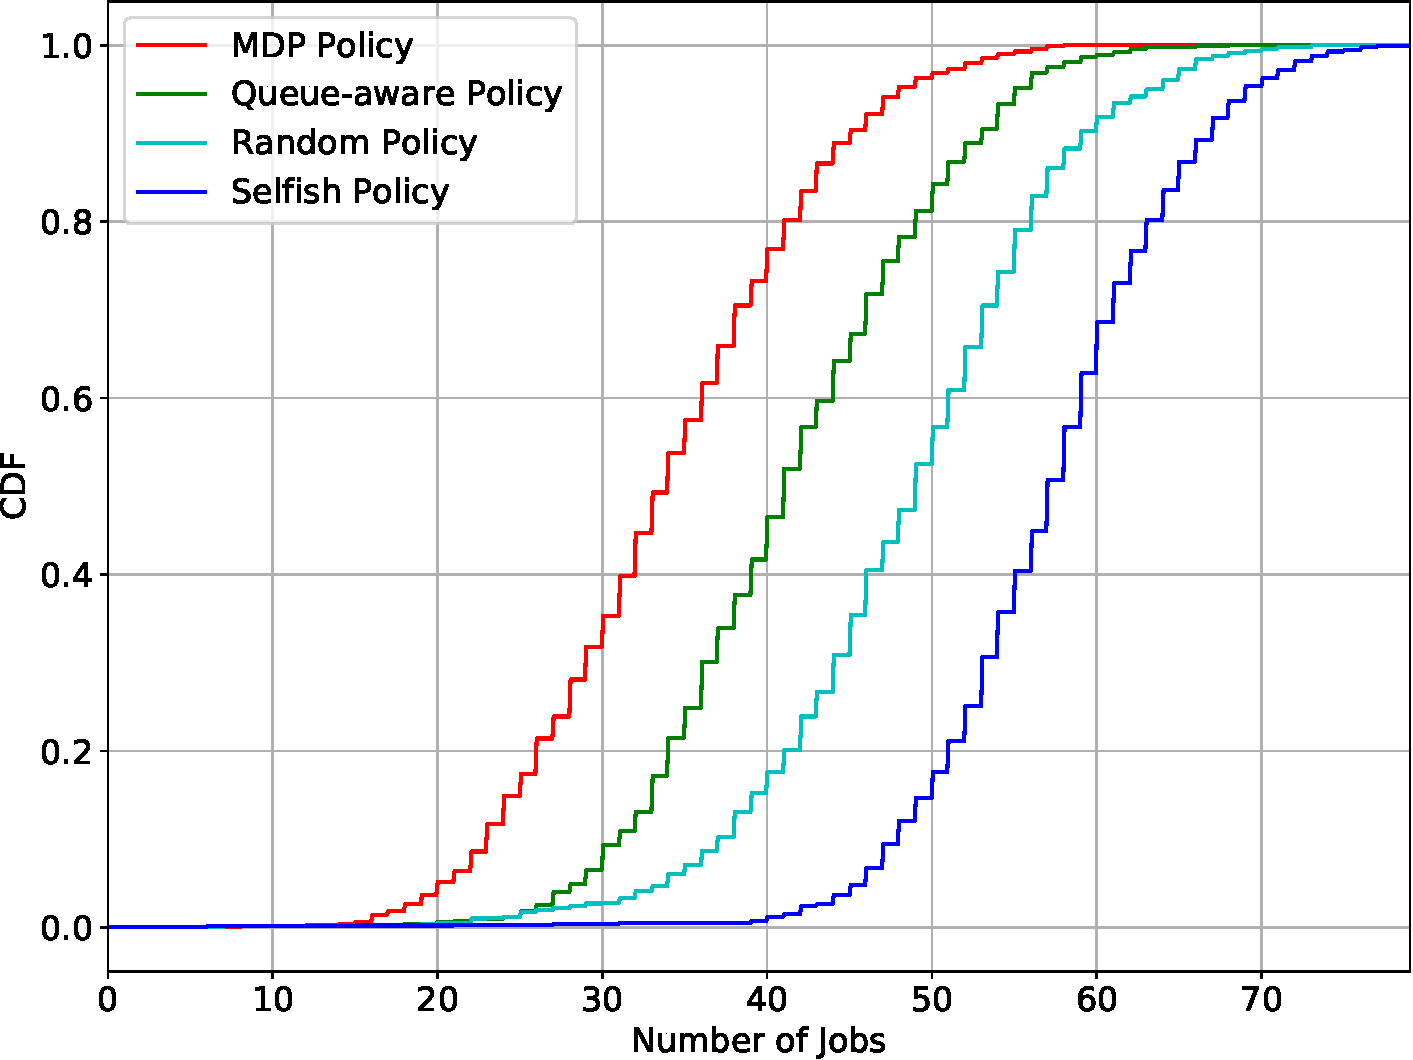
\includegraphics[width=0.30\textwidth]{LowPressure-d1.pdf}&                 %
        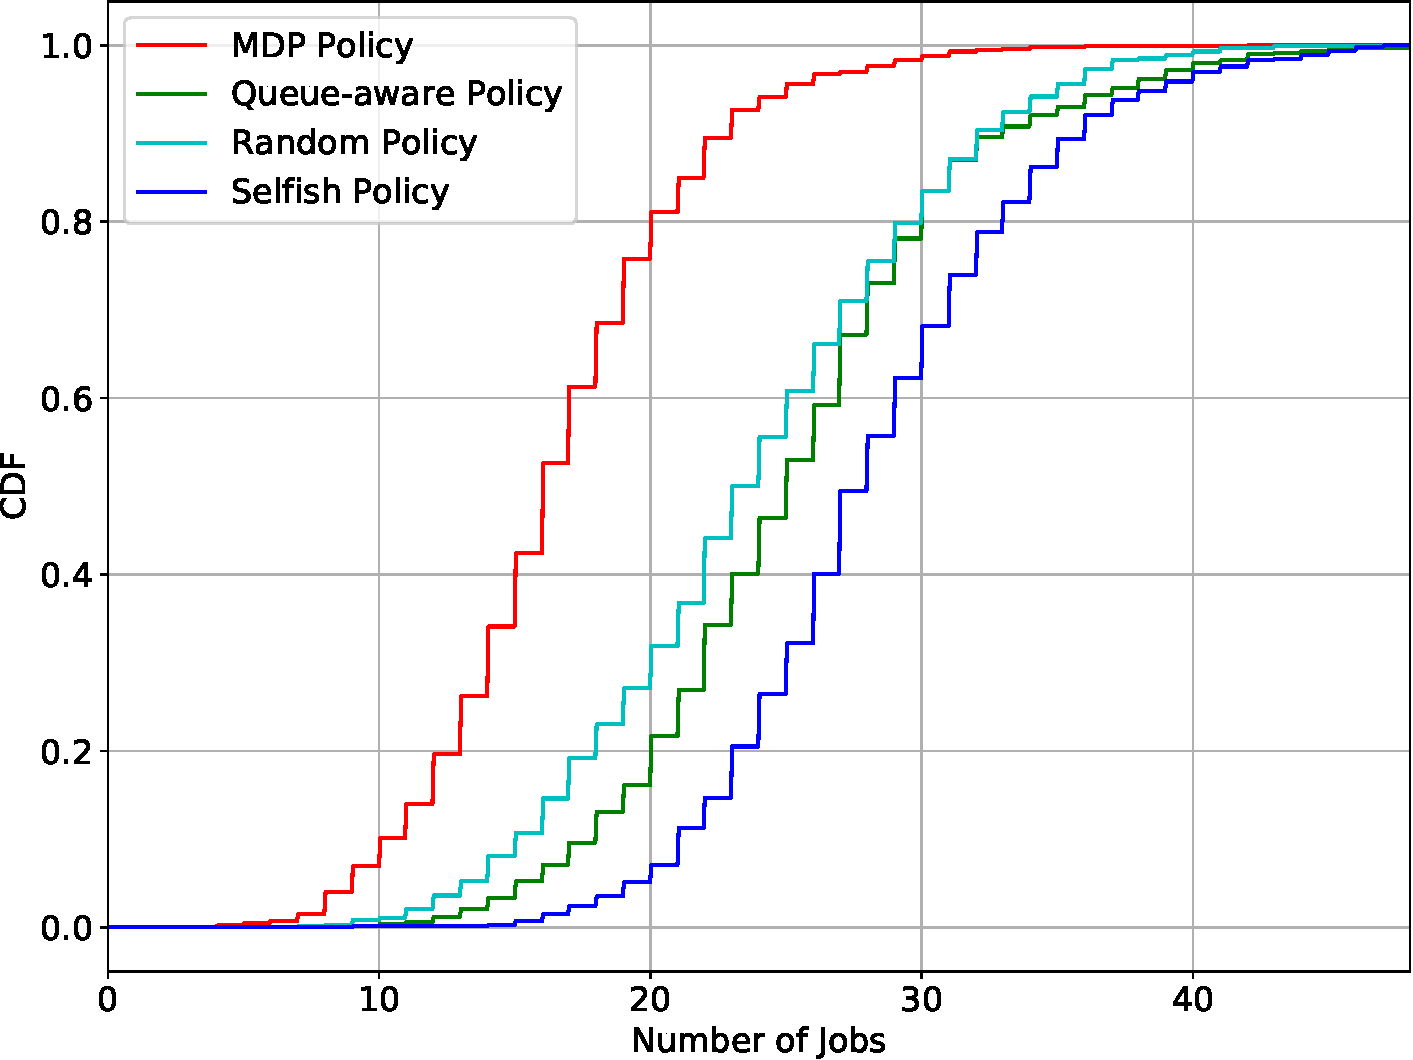
\includegraphics[width=0.30\textwidth]{LowPressure-d2.pdf}                  %
        \\                                                                          %
        {\small (a) Zero \brlatency} &                                                %
        {\small (b) Signaling latency with Support $\set{10,11,\dots,16}$} &
        {\small (c) Maximum \brlatency}                                             %
    \end{tabular}                                                                   %
    \caption{Algorithm Robustness versus Signaling Latency.}
    \label{fig:ss_signal}                                                            %
\end{figure*}                                                                       %
%-----------------------------------------------------------------------------------%

%TODO: tabular the figures here
%-------------------------------------------------------------------%
\begin{figure}[hbt]                                                 %
    \centering                                                      %
    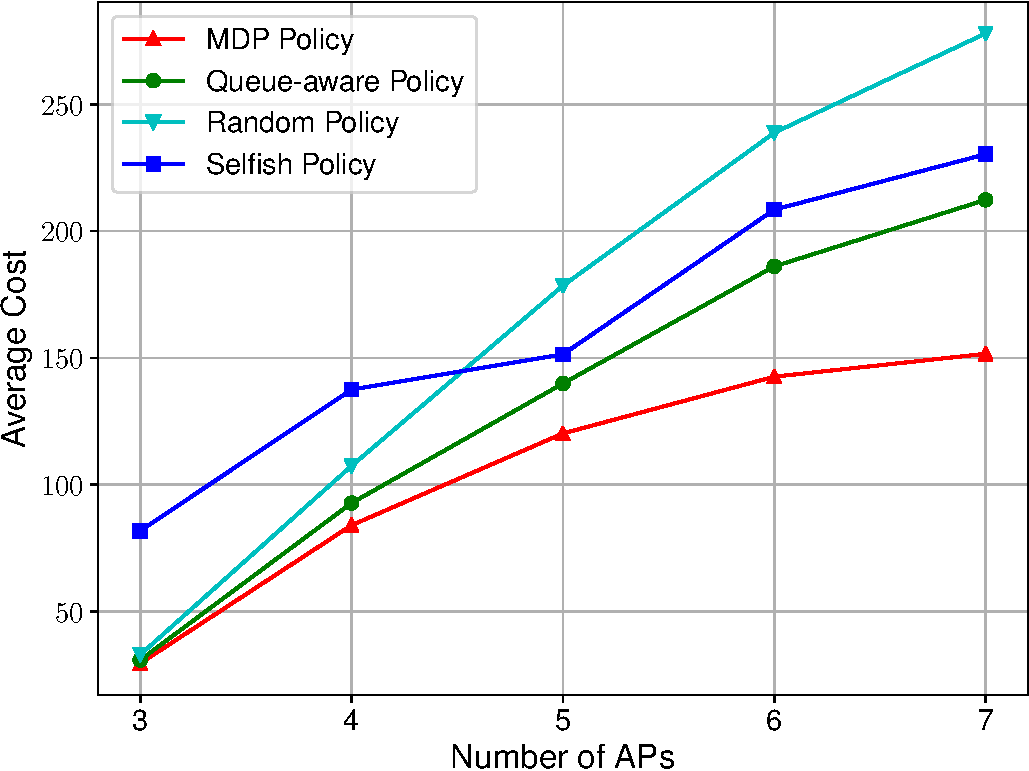
\includegraphics[width=0.45\textwidth]{Study-NumAPs.pdf}        %
    \caption{Illustration of average system cost versus the number of APs.}
    \label{fig:ss_scale}                                            %
\end{figure}                                                        %
%-------------------------------------------------------------------%

%-------------------------------------------------------------------%
\begin{figure}[hbt]                                                 %
    \centering                                                      %
    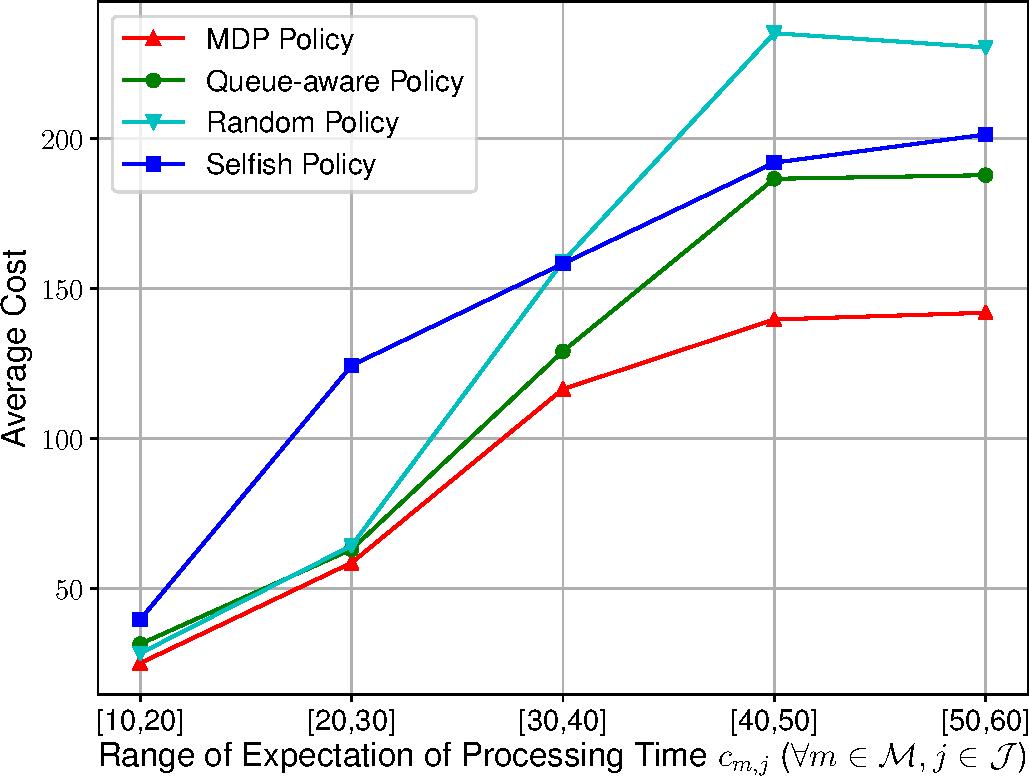
\includegraphics[width=0.45\textwidth]{Study-ProcDist.pdf}      %
    \caption{Illustration of average system cost versus the processing time distributions.}
    \label{fig:ss_dist}                                             %
\end{figure}                                                        %
%-------------------------------------------------------------------%

% %-------------------------------------------------------------------%
% \begin{figure}[hbt]                                                 %
%     \centering                                                      %
%     \includegraphics[width=0.45\textwidth]{bar_graph.pdf}           %
%     \caption{Illustration of impact of penalty factors on algorithms.}
%     \label{fig:ss_penalty}                                          %
% \end{figure}                                                        %
% %-------------------------------------------------------------------%

%NOTE: sensitivity study
\textbf{Signaling Latency.}
The simulation results with different distributions of \brlatency~$\mathcal{D}_{k}$ ($\forall k\in\apSet$) are illustrated in Fig.\ref{fig:ss_signal}, where the cumulative distribution function (CDF) of the job number in the system is plotted.
Specifically, the \brlatency~of all the APs is set to zero and $20$ time slots in Fig.\ref{fig:ss_signal}(a) and Fig.\ref{fig:ss_signal}(c), respectively, and the \brlatency~is a random variable with integer support from $10$ to $16$ time slots in Fig.\ref{fig:ss_signal}(b).
It can be observed from Fig.\ref{fig:ss_signal}(a) and Fig.\ref{fig:ss_signal}(c) that, with the increasing \brlatency, the performance of Queue-aware Policy becomes worse.
It outperforms Random Policy in Fig.5(a) with zero \brlatency~(achieving a smaller number of jobs in the system), and becomes worse in Fig.5(c) with large \brlatency.
This demonstrates that the Queue-aware Policy is sensitive to the \brlatency.
In all the figures, the proposed policy performs better than the benchmarks, which demonstrates the robustness of its performance versus signaling latency.

\textbf{Number of APs.} %(a.k.a arrival rate)
The average system cost versus the number of APs is illustrated in Fig.\ref{fig:ss_scale}.
With the increasing AP numbers, the average system cost increases in all the benchmarks and our proposed policy.
It can be observed that the proposed policy has better performance than the benchmarks for all numbers of APs.
Moreover, the performance gain becomes significant when the computation load is heavy ($K$ is large).
This demonstrates the dispatching efficiency of the proposed policy with heavy load.
On the other hand, the gain is negligible for light load ($K=3$), where the computation capability is sufficient and dispatcher optimization may not be necessary.

\textbf{Processing Time Distributions.}
The simulation results of various distributions of processing time are illustrated in Fig.\ref{fig:ss_dist}, where the $c_{m,j}$ of the processing time distribution $\mathbb{G}(1/c_{m,j})$ ($\forall m\in\esSet,j\in\jSpace$) is generated within different ranges.
Generally speaking, with the increasing average processing time, the average system cost increases in all the benchmarks and our proposed policy.
The simulation results are consistent with that in Fig.\ref{fig:ss_scale}.
It can be observed that the proposed policy has better performance than the benchmarks.
Moreover, the performance gain becomes significant when the computation time is long (the computation load is heavy).
On the other hand, the gain is negligible for short computation time (the computation load is light).

%----------------------------------------------------------------------------------------%
\delete{v20}{
    The CDF of cost is illustrated in Fig.\ref{fig:cdf_cost} where the cost of \emph{SQF policy} is nearly the same as the \emph{selfish policy}, however, the \emph{SQF policy} actually have very poor job departure rate (, throughput) compared with the other's.
    This is because the broadcast information is periodically and outdated, and SQF could not handle the penalty brought by job rejection properly.
    And we take \emph{CDF of number of jobs} other than \emph{CDF of cost} which could better reflect the performance of the average JCT target in the simulation when job rejection considered.
}
\delete{v20.2}{
    As illustrated in Fig.\ref{fig:general_timeline}, the simulation results straightly show that the proposed algorithm outperforms other benchmarks all the time with less pending jobs in the system, and the system converges fast from the start of the time.
    The detailed analysis is provided in Fig.\ref{fig:bar_plot} where three metrics are taken to demonstrate different profiles of the benchmarks.
    Firstly, the \emph{average cost} in Fig.\ref{fig:bar_plot}(a) shows that the proposed algorithm collects less cost than other algorithms within the same time duration.
    % Moreover, 
    Secondly, the \emph{average JCT} of all the jobs in Fig.\ref{fig:bar_plot}(b) resembles the shape of Fig.\ref{fig:bar_plot}(a) which proves the correctness of the cost function selection.
    Finally, The \emph{average throughput} in Fig.\ref{fig:bar_plot}(c) is defined as the division of the total number of computed jobs (i.e., the jobs being accepted by edge servers and finishing the computation) over the time duration, and the results show that the proposed algorithm have the most of jobs computed in the system.
}
%----------------------------------------------------------------------------------------%
    \section{Conclusion}
\label{sec:conclusion}
In this paper, we consider a distributed and asynchronous job dispatching design in an edge computing network residing in a MAN with multiple APs and edge servers.
The APs and edge servers periodically broadcast their local state information to facilitate distributed dispatcher design.
Due to random transmission latency, the system information observed at different dispatchers are asynchronous.
We also consider a practical scenario that not all the state information can be observed by each AP.
We formulate the distributed optimization of job dispatching strategies at all the APs as a POMDP, whose minimization objective is a discount measurement of job delivery and computation time.
We propose a novel low-complexity distributed solution framework based on analytical approximation of value function and one-step policy iteration, where the complicated POMDP solution or value iteration is avoided and the analytical performance lower bound is derived.
The simulation results show that the proposed solution framework outperforms various benchmarks.
In the future work, we shall extend the proposed framework to a more general scenario where the knowledge on the distributions of signaling latency, uploading latency and computation time is absent.
The reinforcement learning would be integrated with the proposed solution framework to address the above issue.
    \section{Research Progress and Future Plan}

\begin{center}
    \begin{tabularx}{0.90\linewidth}{ |c|X| }
        \hline  \textbf{Date}      & \textbf{Targets} \\
        \hline  {2018.09 - 2020.01}  & 
                {Learn the approximation method and low-complexity solution of MDP, formulate the distributed job dispatching problem with outdated information in edge computing network, and submit the paper on the previous content to ICDCS 2020.} \\
        \hline  {2020.01 - 2020.08}  & 
                {Extend the previous work to journal version, and prepare next work in edge computing with new workload with MDP framework.} \\
        \hline  {2020.08 - 2021.02}  & 
                {Learn game theory and computational theory, discover novel metrics and problems in edge storage, and prepare one paper on this to the top-tier conference/journal.} \\
        \hline  {2021.02 - 2021.08}  & 
                {Prepare the skills for intern opportunity or system implementation on large-scale edge/cloud system, and prepare one paper on edge systems.} \\
        \hline  {2020.08 - 2022.07}  & 
                {Publish one work in system work, prepare the thesis and oral defense.} \\
        \hline
    \end{tabularx}
\end{center}

\section{Publications}
\begin{enumerate}
    \item \textbf{Y. Hong}, {B. Lv}, {R. Wang}, {H. Tan}, {Z. Han}, {F.C.M. Lau}, "Distributed Job Dispatching in Edge Computing Networks with Random Uploading Latency: A Low-Complexity POMDP Approach" (submitted to ICDCS 2020)
\end{enumerate}

    % \clearpage
    \bibliographystyle{IEEEtrans}
    \bibliography{references/final.bib}

    % %NOTE: transition matrix and vector for AP
\appendices
\section{ Proof of Lemma \ref{lemma:w_ap} }
\label{append_1}
At the $n$-th time slot of the $t$-th broadcast interval, let $\hat{\vecG{\Theta}}^{(k,\Policy)}_{m,j}(t,n)$ denote the probability vector of job existence under dispatching policy $\Policy$ where the explicit definition is given as follows.
\begin{align}
    \hat{\vecG{\Theta}}^{(k,\Policy)}_{m,j}(t,n) \define \Bracket{
        \hat{\theta}^{(k,\Policy)}_{m,j}(0,t,n),
        \dots,
        \hat{\theta}^{(k,\Policy)}_{m,j}(0,t,n)
    },
\end{align}
where
{\small
\begin{align}
    \hat{\theta}^{(k,\Policy)}_{m,j}(\xi,t,n) \define
    \begin{cases}
        \lambda_{k,j} I[\omega_{k,j}(t)=m], &\xi=0, n < \mathcal{D}_{k}(t)
        \\
        \lambda_{k,j} I[\omega_{k,j}(t+1)=m], &\xi=0, n \geq \mathcal{D}_{k}(t) 
        \\
        \Pr\{R^{(k)}_{m,j}(\xi,t,n)=1\}, & \text{otherwise}
    \end{cases}.
\end{align}
}
The dispatching policy $\Policy$ only affects the first entry of the probability vector, i.e., the arrival probability of one job in the time slot.
Hence, we denote the time-invariant and policy-independent transition matrix $\hat{\Gamma}^{(k)}_{m,j}$ for the state transition on AP between adjacent time slots which is defined below
\begin{align}
    \hat{\Gamma}^{(k)}_{m,j} &\define
    \begin{bmatrix}
        1 & \bar{p}^{(k)}_{m,j,0} &                       &        &                           \\
          & 0                     & \bar{p}^{(k)}_{m,j,1} &        & \text{\huge0}             \\
          &                       & \ddots                & \ddots &                           \\
          & \text{\huge0}         &                       & \ddots & \bar{p}^{(k)}_{m,j,\Xi-1} \\
          &                       &                       &        & 0                         \\
    \end{bmatrix}^{t_B},
\end{align}
where $\bar{p}^{(k)}_{m,j,\xi}$ denotes the probability of job still stay at the $k$-th AP in the next time slot as $\bar{p}^{(k)}_{m,j,\xi} = 1 - p^{(k)}_{m,j,\xi}$, and
\begin{align}
    p^{(k)}_{m,j,\xi} &\define \Pr\{U^{(k)}_{m,j} < (\xi+1) | U^{(k)}_{m,j}>\xi\}
\end{align}
denotes the probability of job offloading to the $m$-th edge server.

Hence, let $\vecG{\Theta}^{(\Policy, k)}_{m,j}(t)$ and $\Gamma^{(k)}_{m,j}$ denotes the probability vector and transition matrix for the adjacent broadcast interval, respectively.
Based on the previous definition in the time slot, the explicit definitions is given as
\begin{align}
    \vecG{\Theta}^{(\Policy, k)}_{m,j}(t) &\define \hat{\vecG{\Theta}}^{(\Policy, k)}_{m,j}(t,0)
    \\
    \vecG{\Theta}^{(k)}_{m,j}(t+1) &= \hat{\vecG{\Theta}}^{(k)}_{m,j}(t, \mathcal{D}_{k}(t)) \times (\hat{\Gamma}^{(k)}_{m,j})^{t_B-\mathcal{D}_{k}(t)},
    \nonumber\\
    \hat{\vecG{\Theta}}^{(k)}_{m,j}(t, \mathcal{D}_{k}(t)) &= \vecG{\Theta}_{m,j}(t) \times (\hat{\Gamma}^{(k)}_{m,j})^{\mathcal{D}_{k}(t)}.
\end{align}
% is composed of two-phase policy separated by $D_k(t)$, which is expressed as follows.

Given that the cost raised on APs is approximated with baseline policy $\Baseline$, the AP (saying the $k$-th AP) would adopt the same dispatching actions as $\Baseline(\Stat(t))$ before and after $\mathcal{D}_{k}(t)$ time slots at the $t$-th broadcast interval.
Hence, we have
\begin{align}
    \vecG{\Theta}^{(k,\Baseline)}_{m,j}(t+1) = \vecG{\Theta}^{(k,\Baseline)}_{m,j}(t) \times (\hat{\Gamma}^{(k)}_{m,j})^{t_B}.
\end{align}
and the transition matrix $\Gamma^{(k)}_{m,j}$ as
\begin{align}
    \Gamma^{(k)}_{m,j} &\define \big( \hat{\Gamma}^{(k)}_{m,j} \big)^{t_B},
\end{align}
and the expression of the cost raised on AP under baseline policy $\Baseline$ is given as follows.
\begin{align}
    &\tilde{W}^{\AP}_{k,m,j}\Paren{\Stat(t+1)} =
    \Inorm{
        \vecG{\Theta}^{(k, \Baseline)}_{m,j}(t+1) \times
        \Bracket{
            \mat{I} - \gamma \Gamma^{(k)}_{m,j}
        }^{-1}
    }.
\end{align}


%NOTE: transition matrix and vector for ES
\section{ Proof of Lemma \ref{lemma:w_es} }
\label{append_2}
The state transition on edge server is composed of both arrival processes of all the APs in the corresponding \emph{potential AP set}, and the departure processes of jobs computation.
We first denote the offloading matrix $\bar{\Gamma}^{(k)}_{m,j}$ for the type-$j$ job offloaded from the $k$-th AP to the $m$-th edge server and the offloading probability vector $\vecG{\rho}^{(k)}_{m,j}({t,n})$ as follows, respectively ($\forall k\in\apSet, m\in\esSet_{k}, j\in\jSpace$).
\begin{align}
    \bar{\Gamma}^{(k)}_{m,j}(t,n) &\define
    \begin{bmatrix}
        0 & p^{(k)}_{m,j,0} &                 &        &                     \\
        & 0                 & p^{(k)}_{m,j,1} &        & \text{\huge0}       \\
        &                   & \ddots          & \ddots &                     \\
        & \text{\huge0}     &                 & \ddots & p^{(k)}_{m,j,\Xi-1} \\
        &                   &                 &        & 1                   \\
    \end{bmatrix},
    \\
    \vecG{\rho}^{(k, \Policy)}_{m,j}({t,n}) &\define \hat{\vecG{\Theta}}^{(k, \Policy)}_{m,j}({t,n}) \times \bar{\Gamma}^{(k)}_{m,j}.
\end{align}
However, the computational complexity of combinations of all the offloading probability vectors for the $m$-th edge server from its \emph{potential AP set} is unacceptable.
To alleviate the complexity, we rewrite the combinatorial arrival process on edge server as an equivalent Bernoulli process with \emph{small probability approximation}, i.e., there would be at most one job arriving in one time slot with the probability as the expected arrival rate of the original combinatorial distribution.
Specifically, the probability distribution of $\sum_{k\in\apSet} \vecG{\rho}^{(k, \Policy)}_{m,j}({t,n})$ is approximated as a Bernoulli distribution with the expected arrival rate denoted as $\hat{\beta}^{\Policy}_{m,j}({t,n})$ whose definition is given as
\begin{align}
    \hat{\beta}^{\Policy}_{m,j}({t,n}) &\define \sum_{k\in\apSet} \sum_{\xi=0,\dots,\Xi-1} \mathbb{E}[\vecG{\rho}^{(k, \Policy)}_{m,j,\xi}({t,n})].
    \label{eqn_0}
\end{align}

%NOTE: transition matrix and vector for Edge Server
Let $\hat{\vecG{\nu}}_{m,j}(t,n)$ denote the probability vector of $Q_{m,j}(t,n)$ at the $n$-th time slot of the $t$-th broadcast interval ($\forall m\in\esSet, j\in\jSpace$)
{\small
\begin{align}
    \vecG{\nu}_{m,j}(t,n) \define \Bracket{
        \Pr\{Q_{m,j}(t,n)=0\}, \dots, \Pr\{Q_{m,j}(t,n)=L_{max}\}
    }.
\end{align}
}
The transition matrix $\hat{\mat{P}}_{m,j}(\hat{\beta}^{\Policy}_{m,j}(t,n))$ for adjacent time slots is determined by $\hat{\beta}^{\Policy}_{m,j}(t,n)$ under policy $\Policy$, whose entries are elaborated as follows.
{\small
\begin{align}
    &\Bracket{ \hat{\mat{P}}_{m,j}(\hat{\beta}^{\Policy}_{m,j}(t,n)) }_{a,b} =
    \nonumber\\
    &\begin{cases}
        (1/c_{m,j})(1-\hat{\beta}^{\Policy}_{m,j}(t,n)), & j=i-1 \\
        (1-1/c_{m,j})\hat{\beta}^{\Policy}_{m,j}(t,n), & j=i+1 \\
        (1/c_{m,j})\hat{\beta}^{\Policy}_{m,j}(t,n) + (1-1/c_{m,j})(1-\hat{\beta}^{\Policy}_{m,j}(t,n)), & i=j \\
        0, &\text{otherwise}
    \end{cases}.
\end{align}
}

Hence, let $\vecG{\nu}_{m,j}(t)$ and $\mat{P}^{\Policy}_{m,j}(t)$ denote the probability vector and transition matrix for adjacent broadcast intervals, respectively.
Based on the previous definitions in the time slot, the explicit definition is given as
\begin{align}
    \vecG{\nu}_{m,j}(t) &\define \hat{\vecG{\nu}}_{m,j}(t,0)
    \\
    \mat{P}^{\Policy}_{m,j}(t) &\define \prod_{n=0,\dots,t_B-1} \hat{\mat{P}}_{m,j}(\hat{\beta}^{\Policy}_{m,j}(t,n)),
    \\
    \vecG{\nu}_{m,j}(t+1) &= \vecG{\nu}_{m,j}(t) \times \mat{P}^{\Policy}_{m,j}(t)
\end{align}

Given that the cost raised on edge servers is approximated with baseline policy $\Baseline$, the transition matrix for state transition is affected by the baseline policy and the system states of APs which could not be decoupled.
\begin{align}
    \mathbb{E}^{\Baseline}[ Q_{m,j}({t+i+1}) | \Stat(t+i)] &\define
        \vecG{\nu}_{m,j}(t) \mat{P}^{\Baseline}_{m,j}(t+i) \vec{h}',
\end{align}
where $\vecG{h} \define [0,1,\dots,L_{max}]$.

Moreover, we notice that under the fixed baseline policy, the arrival process on edge servers would be stationary after the maximum uploading latency from the initial interval and thus the transition matrix is invariant of system states of APs.
Let $\hat{\mat{P}}_{m,j}(\hat{\beta}^{\Baseline}_{m,j}(t,n))$ be the transition matrix for the stationary arrival process under baseline policy $\Baseline$ and
{\small
\begin{align}
    \beta_{m,j}(t,n) &\define \sum_{k\in\apSet} \lambda_{k,j}I[\omega_{k,j}(t)=m] \times \Pr\{ \xi<U_{k,m,j}\le\xi+1 \}
    \nonumber\\
    &= \sum_{k\in\apSet} \lambda_{k,j}I[\omega_{k,j}(t)=m] (\forall n),
\end{align}
}
where $U_{k,m,j}$ denotes the random variable of job uploading latency.

Let
$\mat{P}^{\Baseline}_{m,j}(t) \define \big( \hat{\mat{P}}_{m,j}(\hat{\beta}^{\Baseline}_{m,j}(t,n)) \big)^{t_B}$
denote the transition matrix under baseline policy $\Baseline$ between adjacent broadcast intervals, we could express the cost raised on edge server under baseline policy $\Baseline$ as follows.
{\small
\begin{align}
    &\tilde{W}^{\ES}_{m,j}\Paren{\Stat(t+1)}
    = \sum_{i=0,\dots,\frac{\Xi}{T}} \gamma^{i} \mathbb{E}^{\Baseline}[ Q_{m,j}({t+i+1}) ]
    \nonumber\\
    &~~~~~~~~~~~~+ \gamma^{\frac{\Xi}{T}} 
    \vecG{\nu}({t+\frac{\Xi}{T}+1})
    \Paren{
        \mat{I} - \gamma \mat{P}^{\Baseline}_{m,j}(t)
    }^{-1} \vec{g}',
\end{align}   
}
where $\vec{g}$ is the cost vector taking the definition in equation (\ref{eqn:g_vec}).
%----------------------------------------------------------------------------------------%

\section{ Proof of Lemma \ref{lemma:bound} }
\label{append_3}
The proof is delete due to page limit.

%----------------------------------------------------------------------------------------%

\end{document}